%% LyX 2.4.3 created this file.  For more info, see https://www.lyx.org/.
%% Do not edit unless you really know what you are doing.
\documentclass[12pt,oneside,brazil,normaltoc, sumarioincompleto]{extbook}
\usepackage[T1]{fontenc}
<<<<<<< HEAD
\usepackage[utf8]{inputenc}
=======
\usepackage[latin9]{inputenc}
>>>>>>> 9cc8289ee257736c1a1b3309851f70a5b4b254e3
\usepackage{babel}
\usepackage{array}
\usepackage{float}
\usepackage{makeidx}
\makeindex
\usepackage{graphicx}
\usepackage[a4paper]{geometry}
\geometry{verbose,tmargin=20mm,bmargin=20mm,lmargin=15mm,rmargin=10mm}
\usepackage{fancyhdr}
\pagestyle{fancy}
\usepackage{setspace}
\onehalfspacing
\usepackage[bookmarks=true,bookmarksnumbered=true,bookmarksopen=true,bookmarksopenlevel=1,
 breaklinks=true,pdfborder={0 0 0},pdfborderstyle={},backref=page,colorlinks=false]
 {hyperref}
\hypersetup{pdftitle={Projeto Engenharia: Desenvolvimento Software Aplicado XXXXX},
<<<<<<< HEAD
 pdfauthor={Nome membros equipe; Professor André Duarte Bueno; },
=======
 pdfauthor={Nome membros equipe; Professor Andr� Duarte Bueno; },
>>>>>>> 9cc8289ee257736c1a1b3309851f70a5b4b254e3
 pdfsubject={Descrever assunto},
 pdfkeywords={Copiar do resumo}}

\makeatletter

%%%%%%%%%%%%%%%%%%%%%%%%%%%%%% LyX specific LaTeX commands.
%% Because html converters don't know tabularnewline
\providecommand{\tabularnewline}{\\}

%%%%%%%%%%%%%%%%%%%%%%%%%%%%%% User specified LaTeX commands.
%-----------------------------------------------------------------
<<<<<<< HEAD
% Para incluir formatações especificas para apresentações
%-----------------------------------------------------------------
%https://tex.stackexchange.com/questions/5894/latex-conditional-expression
% Abaixo inserimos o pacote etoolbox que permite a gestão de if..else
=======
% Para incluir formata��es especificas para apresenta��es
%-----------------------------------------------------------------
%https://tex.stackexchange.com/questions/5894/latex-conditional-expression
% Abaixo inserimos o pacote etoolbox que permite a gest�o de if..else
>>>>>>> 9cc8289ee257736c1a1b3309851f70a5b4b254e3
\usepackage{etoolbox}
% Cria o flag
\newtoggle{FormatoApresentacaoTRUE}
\newtoggle{IncluirBibliografiaNoCapituloTRUE}
<<<<<<< HEAD
%Seta o flag - deixe true se for para gerar apresentação de aula e false para formato livro
=======
%Seta o flag - deixe true se for para gerar apresenta��o de aula e false para formato livro
>>>>>>> 9cc8289ee257736c1a1b3309851f70a5b4b254e3
%\toggletrue{FormatoApresentacaoTRUE}
\togglefalse{FormatoApresentacaoTRUE}
%\toggletrue{IncluirBibliografiaNoCapituloTRUE}
\togglefalse{IncluirBibliografiaNoCapituloTRUE}

% Para usar no meio dos arquivos do lyx crie um comando latex e cole o texto abaixo
%\iftoggle{FormatoApresentacaoTRUE}{..verdadeiro..}{..falso..}
%\iftoggle{FormatoApresentacaoTRUE}{\newpage}{}

%---------------------------------------------------------------
<<<<<<< HEAD
% Para adicionar/excluir uma seção inteira
=======
% Para adicionar/excluir uma se��o inteira
>>>>>>> 9cc8289ee257736c1a1b3309851f70a5b4b254e3
%---------------------------------------------------------------
%https://tex.stackexchange.com/questions/193295/lyx-conditional-sections
% Abaixo criamos um novo if
\newif\ifIncluirSecaoProgramacaoAvancada
%\FormatoApresentacaoWidefalse
\IncluirSecaoProgramacaoAvancadatrue
% Para usar
<<<<<<< HEAD
% \ifIncluirSecaoProgramacaoAvancada no início do blobo
=======
% \ifIncluirSecaoProgramacaoAvancada no in�cio do blobo
>>>>>>> 9cc8289ee257736c1a1b3309851f70a5b4b254e3
% \fi para finalizar o bloco

%---------------------------------------------------------------
%GERAL
%---------------------------------------------------------------
\usepackage{verbatim}
%%\usepackage{algorithm}
\usepackage{fancyvrb}
\usepackage{keyval} 
\usepackage{indentfirst}
%\usepackage{color}
\usepackage{xcolor}
\definecolor{azulclaro}{rgb}{0.6,1,1}%   rgb color model
\definecolor{BLACK}{rgb}{0,0,0}%   rgb color model
\definecolor{BLUE}{rgb}{0,0,1}%   rgb color model

%Informa que vai usar o pacote listings, disponibilizado em /usr/share/texmf/doc/latex/styles/listings.dvi
\usepackage{listings}

%Define um novo comando, chamado lst
%observe que lst chama o comando  lstinputlisting.
\newcommand{\lst}[2]{%
    \noindent\rule[-1ex]{\textwidth}{0.3mm}\vspace{-1ex}
    \lstinputlisting[caption={#2},label={#1},stringspaces=false,frame={tb},lineskip=-1pt,extendedchars=true,%
    basicstyle=\footnotesize\tt,labelstep=1,labelstyle=\tiny,indent=2em,language=Java,breaklines]{#1}
    \vspace{1ex}%
}

%\listfiles
%\usepackage[]{hyperref}

%\usepackage{mathptmx}  % instead of package times

%\usepackage[scaled=0.9]{helvet} % or [scaled=0.92], if you like

<<<<<<< HEAD
%% Pacote de citações para formato abnt
=======
%% Pacote de cita��es para formato abnt
>>>>>>> 9cc8289ee257736c1a1b3309851f70a5b4b254e3
%%\usepackage[num]{abntcite}
%%\usepackage[alf]{abntcite}

%%\usepackage[cam,a4,center]{crop}
<<<<<<< HEAD
%% a4 é o tamanho físico
%% center é para centralizar
=======
%% a4 � o tamanho f�sico
%% center � para centralizar
>>>>>>> 9cc8289ee257736c1a1b3309851f70a5b4b254e3
%% cam inclui quatro marcas diferentes

%%\usepackage[cam,width=20truecm,height=28truecm,center]{crop}
%\usepackage[cam,width=18truecm,height=26truecm,center]{crop}

%\noindent

\makeatother

\begin{document}
\begin{center}
{\large UNIVERSIDADE ESTADUAL DO NORTE FLUMINENSE}\\
{\large LABORAT�RIO DE ENGENHARIA E EXPLORA��O DE PETR�LEO}\\
{\large CENTRO DE CI�NCIA E TECNOLOGIA}{\large\par}
\par\end{center}

\begin{center}
{\large}{\large\par}
\par\end{center}

\vspace{3cm}

\begin{center}
{\large PROJETO DE ENGENHARIA}\\
{\large DESENVOLVIMENTO DO SOFTWARE }\\
{\large PoroElasticCalculator}\\
{\large DISCIPLINA : Projeto de Software Aplicado � Engenharia }{\large\par}
\par\end{center}

\vspace{3cm}

\begin{center}
{\large Matheus Bastos \& Nicolau Prates}\\
{\large Prof. Andr� Duarte Bueno}{\large\par}
\par\end{center}

\vspace{5cm}
\thispagestyle{empty}
\begin{center}
{\large MACA� - RJ}\\
{\large Junho - 2025}{\large\par}
\par\end{center}


\tableofcontents{}

\listoffigures

\listoftables

<<<<<<< HEAD
\lhead{\thechapter\space - Especificação}  
\chead{}  
\rhead{}  

\chapter{Concepção\label{chap:Concep=0000E7=0000E3o}\index{Concepção}}

Apresenta-se neste capítulo do projeto de engenharia a concepção,
a especificação do sistema a ser modelado e desenvolvido.
=======
\lhead{\thechapter\space - Especifica��o}  
\chead{}  
\rhead{}  

\chapter{Concep��o\label{chap:Concep=0000E7=0000E3o}\index{Concep��o}}

Apresenta-se neste cap�tulo do projeto de engenharia a concep��o,
a especifica��o do sistema a ser modelado e desenvolvido.
>>>>>>> 9cc8289ee257736c1a1b3309851f70a5b4b254e3


\section{Metodologia\label{sec:Metodologia}}

A Figura \ref{fig: Metodologia utilizada no desenvolvimento do sistema}
apresenta a metodologia a ser utilizada no desenvolvimento do sistema.
\begin{figure}[ph]
\begin{centering}
<<<<<<< HEAD
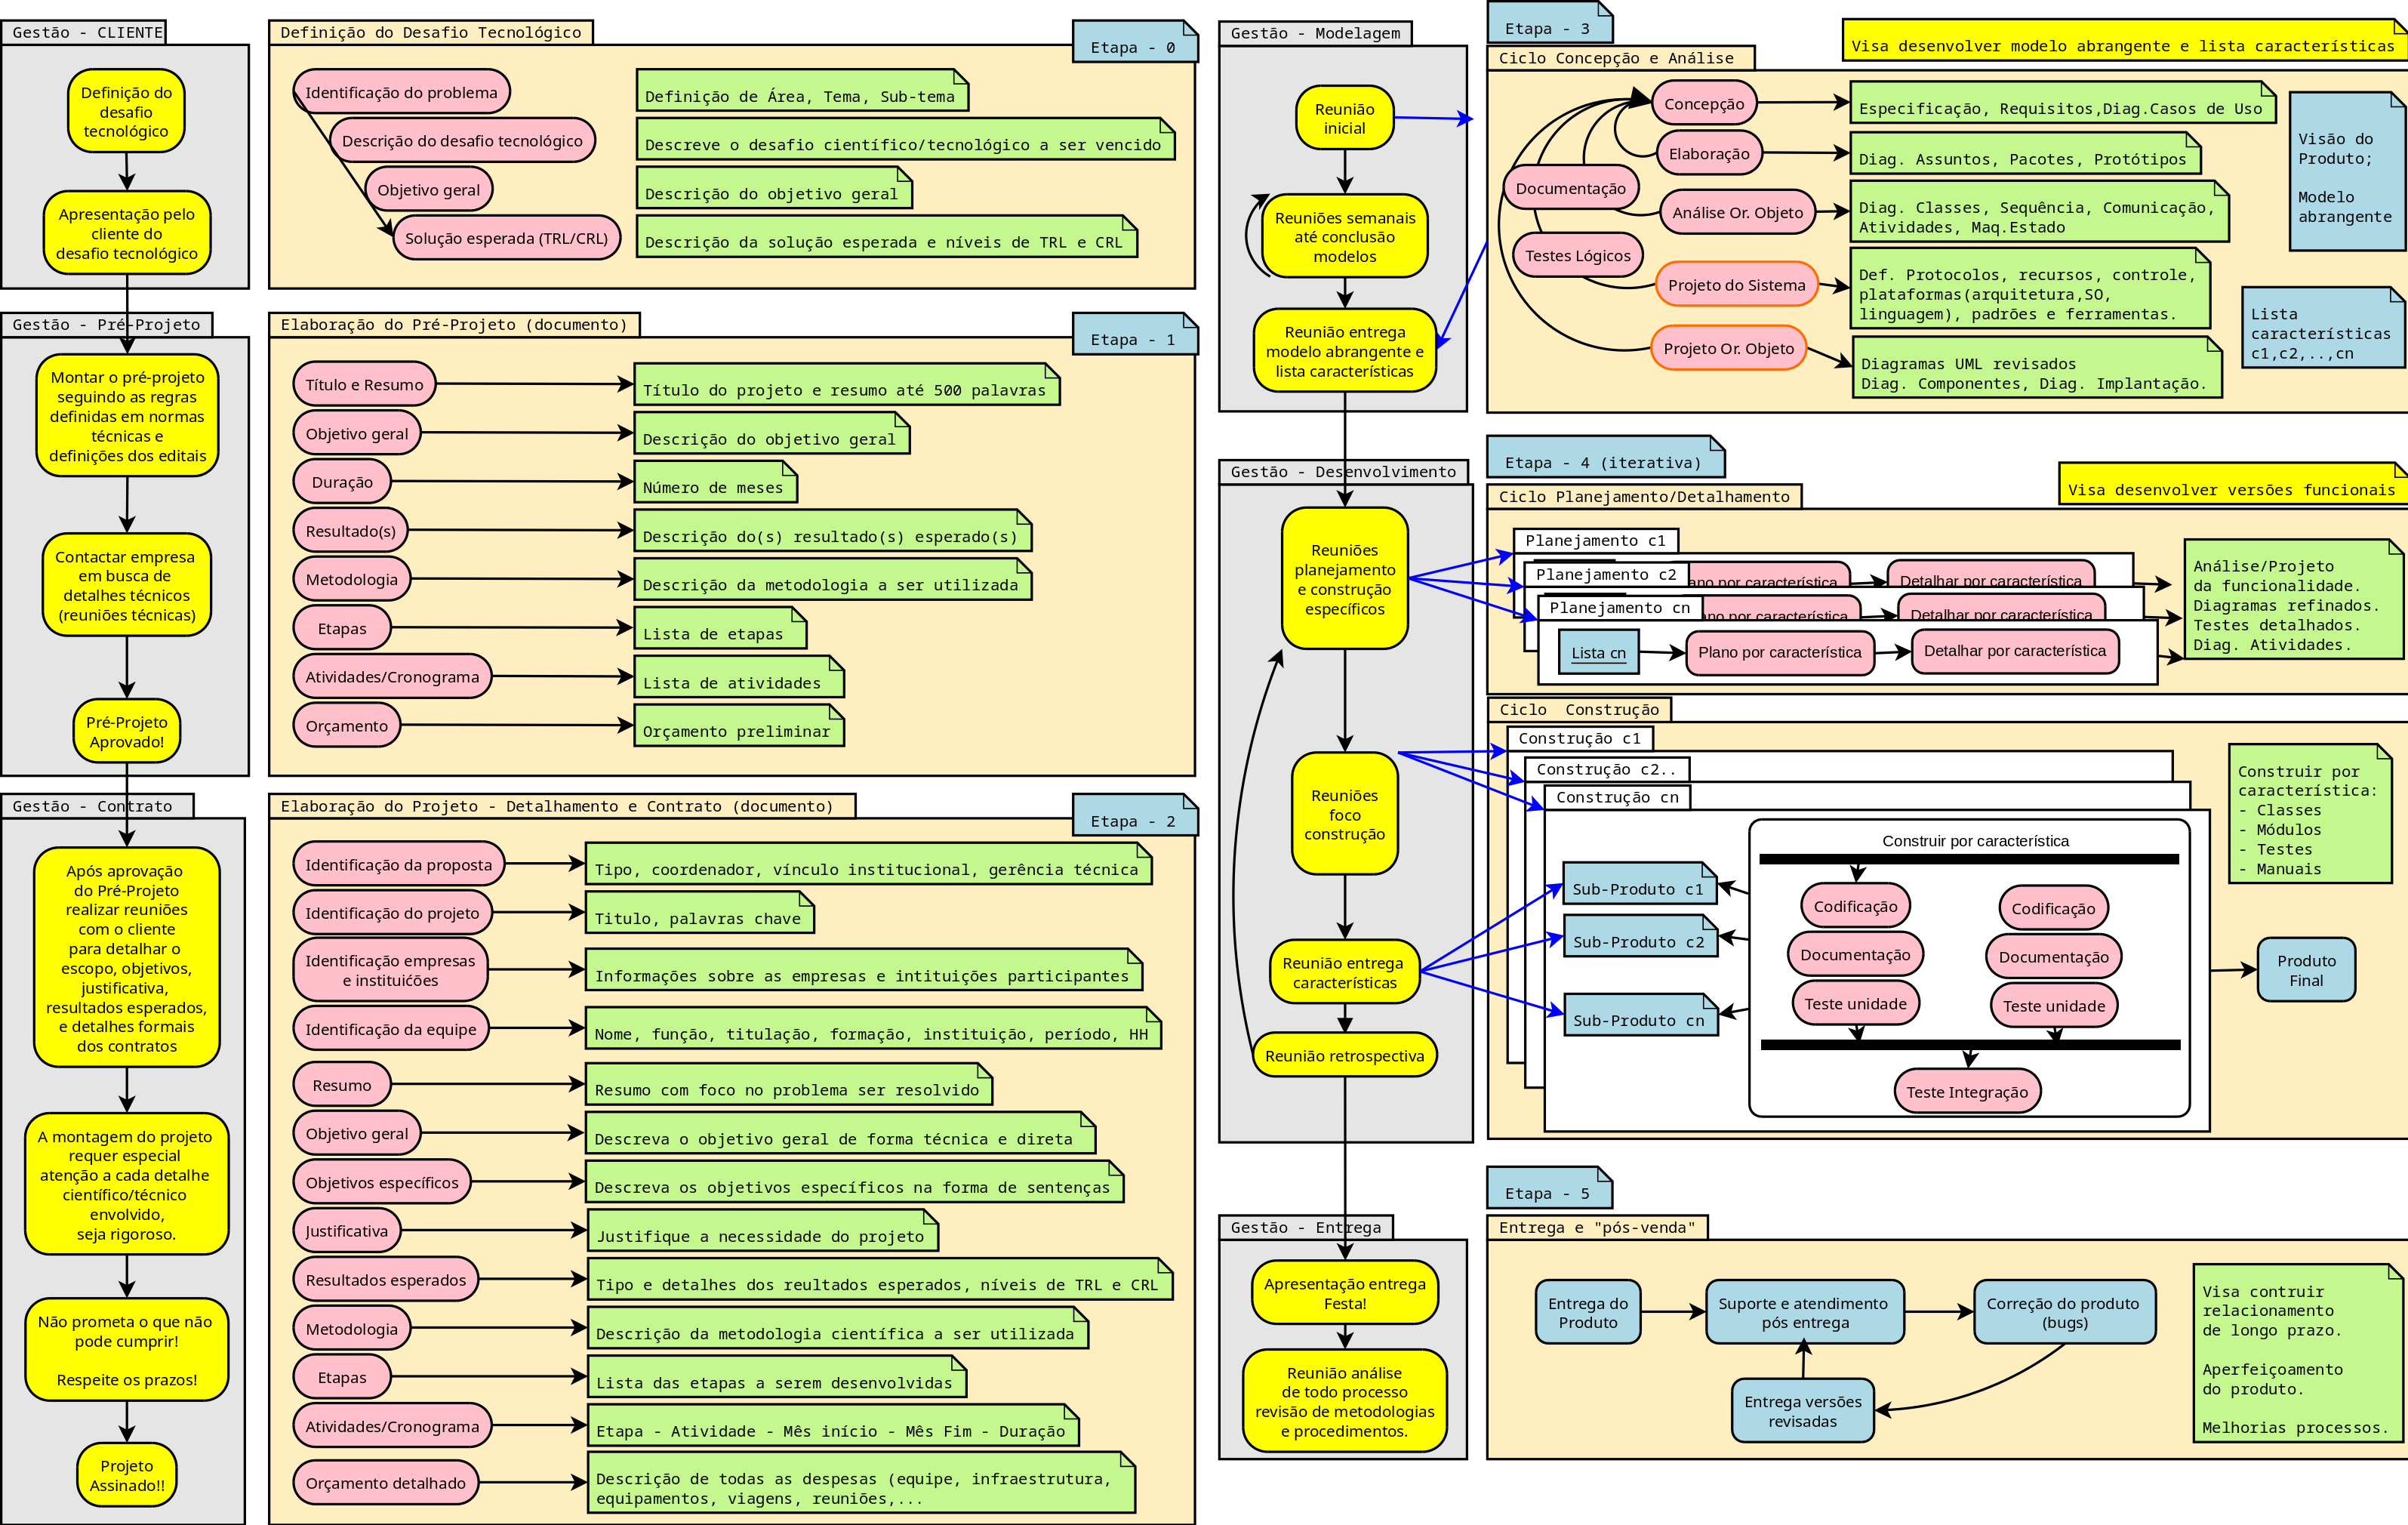
\includegraphics[width=1\textwidth,keepaspectratio,height=0.8\textheight]{imagens/ProjetoEngenharia-Etapas-Geral-wide.png}
=======

\includegraphics[width=1\textwidth,keepaspectratio,height=0.8\textheight]{../../imagens/ProjetoEngenharia-Etapas-Geral-wide}
>>>>>>> 9cc8289ee257736c1a1b3309851f70a5b4b254e3
\par\end{centering}
\caption{Metodologia utilizada no desenvolvimento do sistema\label{fig: Metodologia utilizada no desenvolvimento do sistema}}
\end{figure}


\section{Nome do Sistema/Produto\label{sec: Nome do sistema/produto}}

\begin{tabular*}{14cm}{@{\extracolsep{\fill}}|c|>{\centering}p{8cm}|}
\hline 
\textbf{Nome} & \tabularnewline
\hline 
\textbf{Componentes principais} & \tabularnewline
\hline 
<<<<<<< HEAD
\textbf{Missão} & \tabularnewline
\hline 
\end{tabular*}

\section{Especificação\label{sec:Especifica=0000E7=0000E3o}\index{Especificação}\index{especificação}}

Apresenta-se a seguir a especificação do software.

....coloque aqui a especificação...

...eventualmente coloque imagem ilustrativa geral, mostrando o que
se pretente (primeira ideia) do software; normalmente esta figura
já será mais detalhada que aquela apresentada no escopo...

\section{Requisitos\index{Requisitos}\label{sec:Requisitos} }

Apresenta-se nesta seção os requisitos funcionais e não funcionais.
=======
\textbf{Miss�o} & \tabularnewline
\hline 
\end{tabular*}

\section{Especifica��o\label{sec:Especifica=0000E7=0000E3o}\index{Especifica��o}\index{especifica��o}}

Apresenta-se a seguir a especifica��o do software.

....coloque aqui a especifica��o...

...eventualmente coloque imagem ilustrativa geral, mostrando o que
se pretente (primeira ideia) do software; normalmente esta figura
j� ser� mais detalhada que aquela apresentada no escopo...

\section{Requisitos\index{Requisitos}\label{sec:Requisitos} }

Apresenta-se nesta se��o os requisitos funcionais e n�o funcionais.
>>>>>>> 9cc8289ee257736c1a1b3309851f70a5b4b254e3

\subsection{Requisitos funcionais\index{Requisitos funcionais}\label{subsec:Requisitos-funcionais}}

Apresenta-se a seguir os requisitos funcionais.

\begin{tabular*}{14cm}{@{\extracolsep{\fill}}|c|p{11.5cm}|}
\hline 
<<<<<<< HEAD
\textbf{RF-01} & O sistema deve conter uma base de dados xxx. O usuário deve ser capaz
=======
\textbf{RF-01} & O sistema deve conter uma base de dados xxx. O usu�rio deve ser capaz
>>>>>>> 9cc8289ee257736c1a1b3309851f70a5b4b254e3
de xxx.\tabularnewline
\hline 
\end{tabular*}

\bigskip{}
\begin{tabular*}{14cm}{@{\extracolsep{\fill}}|c|p{11.5cm}|}
\hline 
<<<<<<< HEAD
\textbf{RF-02} & O usuário deverá ter liberdade para xxxx.\tabularnewline
=======
\textbf{RF-02} & O usu�rio dever� ter liberdade para xxxx.\tabularnewline
>>>>>>> 9cc8289ee257736c1a1b3309851f70a5b4b254e3
\hline 
\end{tabular*}

\bigskip{}
\begin{tabular*}{14cm}{@{\extracolsep{\fill}}|c|p{11.5cm}|}
\hline 
\textbf{RF-03} & Deve permitir o carregamento de arquivos criados pelo software.\tabularnewline
\hline 
\end{tabular*}

\bigskip{}

\begin{tabular*}{14cm}{@{\extracolsep{\fill}}|c|p{11.5cm}|}
\hline 
<<<<<<< HEAD
\textbf{RF-04} & Deve permitir a escolha da equação xxx.\tabularnewline
=======
\textbf{RF-04} & Deve permitir a escolha da equa��o xxx.\tabularnewline
>>>>>>> 9cc8289ee257736c1a1b3309851f70a5b4b254e3
\hline 
\end{tabular*}

\bigskip{}

\begin{tabular*}{14cm}{@{\extracolsep{\fill}}|c|p{11.5cm}|}
\hline 
<<<<<<< HEAD
\textbf{RF-05} & O usuário deve ter tal liberdade para escolher xxx.\tabularnewline
=======
\textbf{RF-05} & O usu�rio deve ter tal liberdade para escolher xxx.\tabularnewline
>>>>>>> 9cc8289ee257736c1a1b3309851f70a5b4b254e3
\hline 
\end{tabular*}

\bigskip{}
\begin{tabular*}{14cm}{@{\extracolsep{\fill}}|c|p{11.5cm}|}
\hline 
<<<<<<< HEAD
\textbf{RF-06} & O usuário poderá plotar seus resultados em um gráfico. O gráfico poderá
=======
\textbf{RF-06} & O usu�rio poder� plotar seus resultados em um gr�fico. O gr�fico poder�
>>>>>>> 9cc8289ee257736c1a1b3309851f70a5b4b254e3
ser salvo como imagem ou ter seus dados exportados como texto.\tabularnewline
\hline 
\end{tabular*}

\bigskip{}


<<<<<<< HEAD
\subsection{Requisitos não funcionais\index{Requisitos não funcionais}\label{subsec:Requisitos-n=0000E3o-funcionais}}

\begin{tabular*}{14cm}{@{\extracolsep{\fill}}|c|p{11cm}|}
\hline 
\textbf{RNF-01} & Os cálculos devem ser feitos utilizando-se xxxx.\tabularnewline
=======
\subsection{Requisitos n�o funcionais\index{Requisitos n�o funcionais}\label{subsec:Requisitos-n=0000E3o-funcionais}}

\begin{tabular*}{14cm}{@{\extracolsep{\fill}}|c|p{11cm}|}
\hline 
\textbf{RNF-01} & Os c�lculos devem ser feitos utilizando-se xxxx.\tabularnewline
>>>>>>> 9cc8289ee257736c1a1b3309851f70a5b4b254e3
\hline 
\end{tabular*}

\bigskip{}

\begin{tabular*}{14cm}{@{\extracolsep{\fill}}|c|p{11cm}|}
\hline 
<<<<<<< HEAD
\textbf{RNF-02} & O programa deverá ser multi-plataforma, podendo ser executado em \emph{Windows},
=======
\textbf{RNF-02} & O programa dever� ser multi-plataforma, podendo ser executado em \emph{Windows},
>>>>>>> 9cc8289ee257736c1a1b3309851f70a5b4b254e3
\emph{GNU/Linux} ou \emph{Mac}.\tabularnewline
\hline 
\end{tabular*}


\section{Casos de Uso\label{sec:Casos-de-uso}\index{Casos de uso} }

<<<<<<< HEAD
A Tabela \ref{cap:Exemplo-de-um-caso-de-uso (tabela)} mostra a descrição
=======
A Tabela \ref{cap:Exemplo-de-um-caso-de-uso (tabela)} mostra a descri��o
>>>>>>> 9cc8289ee257736c1a1b3309851f70a5b4b254e3
de um caso de uso.

\begin{table}[H]
\caption{Caso de uso 1\label{cap:Exemplo-de-um-caso-de-uso (tabela)}}

~
\centering{}%
\begin{tabular}{|c|p{10cm}|}
\hline 
Nome do caso de uso: & \tabularnewline
\hline 
\hline 
<<<<<<< HEAD
Resumo/descrição: & \tabularnewline
=======
Resumo/descri��o: & \tabularnewline
>>>>>>> 9cc8289ee257736c1a1b3309851f70a5b4b254e3
\hline 
Etapas: & \tabularnewline
\hline 
\hline 
<<<<<<< HEAD
Cenários alternativos: & \tabularnewline
=======
Cen�rios alternativos: & \tabularnewline
>>>>>>> 9cc8289ee257736c1a1b3309851f70a5b4b254e3
\hline 
\end{tabular}
\end{table}


\subsection{Diagrama de caso de uso geral\label{subsec: Diagrama de caso de uso geral}}

<<<<<<< HEAD
....coloque aqui caso de uso geral, descrição + figura(s)...
=======
....coloque aqui caso de uso geral, descri��o + figura(s)...
>>>>>>> 9cc8289ee257736c1a1b3309851f70a5b4b254e3

exemplo...

O diagrama de caso de uso geral da Figura \ref{cap:Diagrama-caso-uso-geral}
<<<<<<< HEAD
mostra o usuário acessando os sistemas de ajuda do software, calculando
a área de uma função ou analisando resultados. 
=======
mostra o usu�rio acessando os sistemas de ajuda do software, calculando
a �rea de uma fun��o ou analisando resultados. 
>>>>>>> 9cc8289ee257736c1a1b3309851f70a5b4b254e3

\begin{figure}[ph]
\begin{centering}

\includegraphics[width=1\textwidth,keepaspectratio,height=0.3\textheight]{imagens/DiagramaDeCasoUso-Geral}
\par\end{centering}
\caption{Diagrama de caso de uso -- Caso de uso geral\label{cap:Diagrama-caso-uso-geral}}
\end{figure}


<<<<<<< HEAD
\subsection{Diagrama de caso de uso específico\label{subsec: Diagrama de caso de uso espec=0000EDfico}}

....coloque aqui casos de uso específicos, descrição + figura(s)...

exemplo...O caso de uso Calcular área função descrito na Figura \ref{cap:Diagrama-caso-uso-geral}
e na Tabela \ref{cap:Exemplo-de-um-caso-de-uso (tabela)} é detalhado
na Figura \ref{cap:Diagrama-de-caso-de-uso-especifico:Titulo}. O
usuário criará um objeto função matemática, um objeto para sua integração;
em seguida, definirá o intervalo de integração, calculará a área da
função criada e,  por fim, analisará os resultados (eventualmente
gerará gráficos com os resultados obtidos utilizando um sistema externo,
como o software \emph{gnuplot}). Este diagrama de caso de uso ilustra
as etapas a serem executadas pelo usuário ou sistema, a iteração do
usuário com o sistema.
=======
\subsection{Diagrama de caso de uso espec�fico\label{subsec: Diagrama de caso de uso espec=0000EDfico}}

....coloque aqui casos de uso espec�ficos, descri��o + figura(s)...

exemplo...O caso de uso Calcular �rea fun��o descrito na Figura \ref{cap:Diagrama-caso-uso-geral}
e na Tabela \ref{cap:Exemplo-de-um-caso-de-uso (tabela)} � detalhado
na Figura \ref{cap:Diagrama-de-caso-de-uso-especifico:Titulo}. O
usu�rio criar� um objeto fun��o matem�tica, um objeto para sua integra��o;
em seguida, definir� o intervalo de integra��o, calcular� a �rea da
fun��o criada e,  por fim, analisar� os resultados (eventualmente
gerar� gr�ficos com os resultados obtidos utilizando um sistema externo,
como o software \emph{gnuplot}). Este diagrama de caso de uso ilustra
as etapas a serem executadas pelo usu�rio ou sistema, a itera��o do
usu�rio com o sistema.
>>>>>>> 9cc8289ee257736c1a1b3309851f70a5b4b254e3

\begin{figure}[ph]
\begin{centering}
\includegraphics[width=1\textwidth]{imagens/DiagramaDeCasoDeUso-Especifico-1}
\par\end{centering}
<<<<<<< HEAD
\caption{Diagrama de caso de uso específico -- Título\label{cap:Diagrama-de-caso-de-uso-especifico:Titulo}}
\end{figure}

%\begin{description}
%\item [{Nota:}] ~\\
Não perca de vista a visão do todo; do projeto de engenharia como
um todo. Cada capítulo, cada seção, cada parágrafo deve se encaixar.
Este é um diferencial fundamental do engenheiro em relação ao técnico,
a capacidade de desenvolver projetos, de ver o todo e suas diferentes
partes, de modelar processos/sistemas/produtos de engenharia.
%\end{description}
=======
\caption{Diagrama de caso de uso espec�fico -- T�tulo\label{cap:Diagrama-de-caso-de-uso-especifico:Titulo}}
\end{figure}

\begin{description}
\item [{Nota:}] ~\\
N�o perca de vista a vis�o do todo; do projeto de engenharia como
um todo. Cada cap�tulo, cada se��o, cada par�grafo deve se encaixar.
Este � um diferencial fundamental do engenheiro em rela��o ao t�cnico,
a capacidade de desenvolver projetos, de ver o todo e suas diferentes
partes, de modelar processos/sistemas/produtos de engenharia.
\end{description}
>>>>>>> 9cc8289ee257736c1a1b3309851f70a5b4b254e3



\lhead{\thechapter\space - Elabora��o}  

\chapter{Elabora��o\index{Elabora��o}\label{sec:Elabora=0000E7=0000E3o}}

Depois da defini��o dos objetivos, da especifica��o do software e
da montagem dos primeiros diagramas de caso de uso, a equipe de desenvolvimento
do projeto de engenharia passa por um processo de elabora��o que envolve
o estudo de conceitos relacionados ao sistema a ser desenvolvido,
a an�lise de dom�nio e a identifica��o de pacotes. 

Na elabora��o fazemos uma an�lise dos requisitos, ajustando os requisitos
iniciais de forma a desenvolver um sistema �til, que atenda �s necessidades
do usu�rio e, na medida do poss�vel, permita seu reuso e futura extens�o.

Eliminam-se os requisitos \textquotedbl imposs�veis\textquotedbl{}
e ajusta-se a id�ia do sistema de forma que este seja flex�vel, considerando-se
aspectos como custos e prazos.

\section{An�lise de dom�nio\label{sec:An=0000E1lise-de-dom=0000EDnio}}

Ap�s estudo dos requisitos/especifica��es do sistema, algumas entrevistas,
estudos na biblioteca e disciplinas do curso foi poss�vel identificar
nosso dom�nio de trabalho:
\begin{itemize}
\item Defini��o e caracteriza��o do dom�nio a ser investigado 
\item Descri��o das �reas/disciplinas relacionadas.
\item Descri��o de quest�es associadas a espa�o/tempo (espa�o f�sico, local,
instala��o).
\item Fotografias de sistemas equivalentes/parecidos.
\item ...
\end{itemize}

\section{Formula��o te�rica\label{sec:Formula=0000E7=0000E3o-te=0000F3rica}}

...coloque aqui texto explicando a formula��o f�sica-matem�tica, a
descri��o das equa��es que ser�o utilizadas...

...aqui entram figuras, tabelas explicativas, equa��es a serem utilizadas
no software...

...logo depois, com os dados levantados na an�lise de dom�nio, e esta
formula��o te�rica, iremos identificar os pacotes, os assuntos com
os quais iremos trabalhar...

... no final da formula��o te�rica, indicar livros e artigos que tem
mais informa��o sobre o assunto...

...se vai usar modelos num�ricos, colocar se��o 3.3.x falando deles;
no final citar/referenciar fontes...

\section{Identifica��o de pacotes -- assuntos}

...aqui...
\begin{itemize}
\item Nome Pacote: Descri��o. O que �, para que serve, como se relaciona
com os demais pacotes.
\item Nome Pacote: Descri��o. O que �, para que serve, como se relaciona
com os demais pacotes.
\item Nome Pacote: Descri��o. O que �, para que serve, como se relaciona
com os demais pacotes.
\end{itemize}

\section{Diagrama de pacotes -- assuntos\label{sec: Diagrama de pacotes =002013 assuntos}}

...aqui...

coloque aqui texto falando do diagrama de pacotes, referencie a figura.
Veja Figura \ref{fig:Diagrama-de-Pacotes}.

\begin{figure}[H]
\begin{centering}

\includegraphics[width=1\textwidth]{imagens/DiagramaDeComponentes-Assuntos-Pacotes}
\par\end{centering}
\caption{Diagrama de Pacotes\label{fig:Diagrama-de-Pacotes}}
\end{figure}

\begin{description}
\item [{Nota:}] ~\\
N�o perca de vista a vis�o do todo; do projeto de engenharia como
um todo. Cada cap�tulo, cada se��o, cada par�grafo deve se encaixar.
Este � um diferencial fundamental do engenheiro em rela��o ao t�cnico,
a capacidade de desenvolver projetos, de ver o todo e suas diferentes
partes, de modelar processos/sistemas/produtos de engenharia.
\end{description}



\lhead{\thechapter\space - Análise Orientada a Objeto}  

\chapter{AOO\index{AOO} -- Análise Orientada a Objeto\label{chap:An=0000E1lise Orientada a Objeto}\index{Análise orientada a objeto}\label{sec:AOO}}



\section{Diagramas de classes\label{sec:Diagramas-de-classes}}

O diagrama de classes é apresentado na Figura \ref{cap:Diagrama-de-classes}. 

\begin{figure}[H]
\begin{centering}
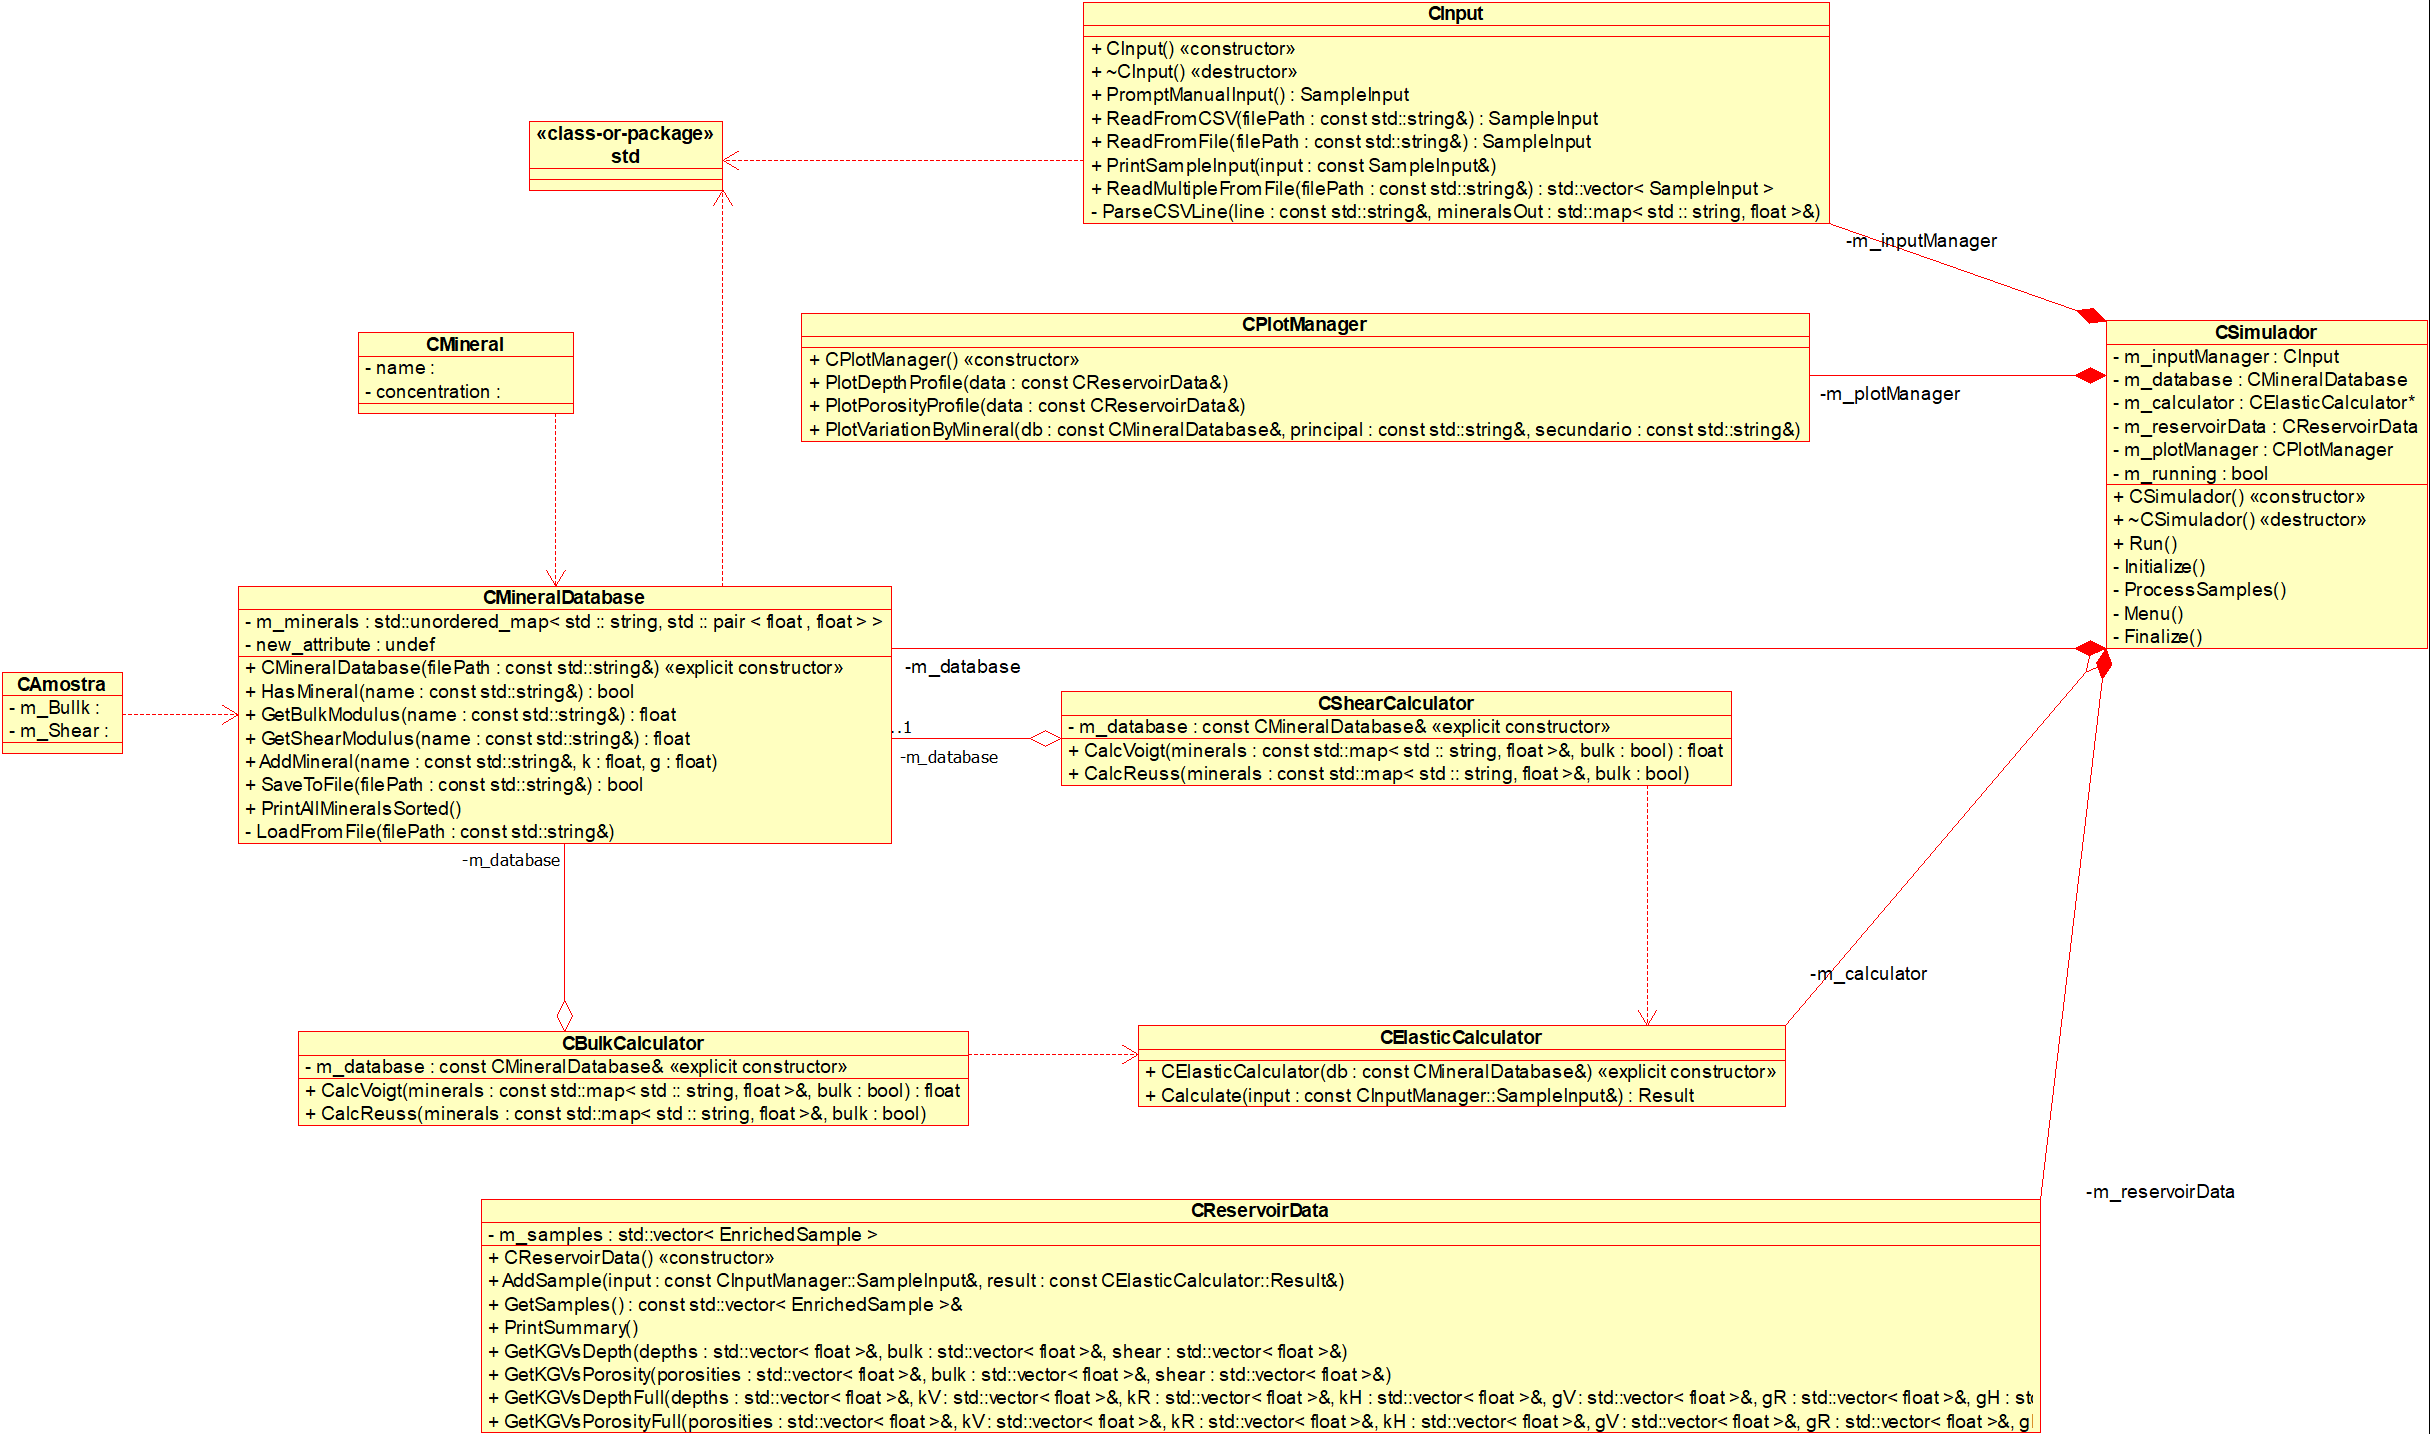
\includegraphics[width=1.0\textwidth]{imagens/Classes.png }
\par\end{centering}
\caption{Diagrama de classes\label{cap:Diagrama-de-classes}}
\end{figure}


\subsection{Dicionário de classes\label{subsec:Dicion=0000E1rio-de-classes}}

\begin{itemize}
    \item \textbf{CSimulator}
    \begin{description}
        \item[Responsabilidade:] Classe principal que orquestra a execução do programa. É responsável por inicializar todos os componentes, gerenciar o menu de interação com o usuário e controlar o fluxo de dados entre os módulos de entrada, cálculo e visualização.
        
        \item[Atributos:] 
        \begin{itemize}
            \item \texttt{-m\_input}: \texttt{CInput} – Instância do gerenciador de entrada de dados.
            \item \texttt{-m\_database}: \texttt{CMineralDatabase} – Instância do banco de dados de minerais.
            \item \texttt{-m\_calculator}: \texttt{CElasticCalculator} – Instância do módulo de cálculo de propriedades elásticas.
            \item \texttt{-m\_reservoirData}: \texttt{CReservoirData} – Instância do repositório de dados das amostras processadas.
            \item \texttt{-m\_plotManager}: \texttt{CPlotManager} – Instância do gerenciador de visualização gráfica.
        \end{itemize}
        
        \item[Métodos:]
        \begin{itemize}
            \item \texttt{+CSimulator() / +\~CSimulator()}: Construtor e destrutor da classe.
            \item \texttt{+Run()}: Inicia e gerencia o laço de execução principal da aplicação.
            \item \texttt{-Initialize()}: Prepara e aloca os recursos para os módulos do sistema.
            \item \texttt{-Menu()}: Exibe as opções disponíveis e captura a escolha do usuário.
            \item \texttt{-ProcessSamples()}: Dispara o fluxo de processamento para uma nova amostra.
            \item \texttt{-Finalize()}: Libera os recursos alocados antes de encerrar a aplicação.
        \end{itemize}
    \end{description}

    \item \textbf{CInput}
    \begin{description}
        \item[Responsabilidade:] Gerencia a aquisição de dados das amostras, seja por meio de entrada manual do usuário no console ou pela leitura e interpretação de arquivos de dados formatados.
        
        \item[Métodos:]
        \begin{itemize}
            \item \texttt{+CInput() / +\~CInput()}: Construtor e destrutor da classe.
            \item \texttt{+PromptManualInput()}: Solicita interativamente os dados da amostra ao usuário.
            \item \texttt{+ReadFromCSV()}: Lê dados de um arquivo no formato CSV (não utilizado na versão final).
            \item \texttt{+ReadFromFile()}: Lê os dados de uma única amostra de um arquivo de texto.
            \item \texttt{+PrintSampleInput()}: Exibe os dados de entrada de uma amostra no console para verificação.
            \item \texttt{+ReadMultipleFromFile()}: Lê uma ou mais amostras de um arquivo de texto.
            \item \texttt{-ParseCSVLine()}: Interpreta uma única linha de um arquivo de dados para extrair a composição mineralógica.
        \end{itemize}
    \end{description}

    \item \textbf{CMineralDatabase}
    \begin{description}
        \item[Responsabilidade:] Encapsula o acesso à base de dados de minerais. É responsável por carregar, salvar e fornecer as propriedades elásticas (módulo de compressibilidade e de cisalhamento) de cada mineral.
        
        \item[Atributos:]
        \begin{itemize}
            \item \texttt{-m\_minerals}: Estrutura de dados que armazena as propriedades dos minerais carregados em memória.
            \item \texttt{-m\_databaseFilePath}: Caminho para o arquivo físico da base de dados.
        \end{itemize}
        
        \item[Métodos:]
        \begin{itemize}
            \item \texttt{+CMineralDatabase(filePath)}: Construtor que inicializa o objeto e carrega os dados do arquivo especificado.
            \item \texttt{+HasMineral(name)}: Verifica a existência de um mineral na base de dados.
            \item \texttt{+GetBulkModulus(name)}: Retorna o módulo de compressibilidade (K) de um mineral.
            \item \texttt{+GetShearModulus(name)}: Retorna o módulo de cisalhamento (G) de um mineral.
            \item \texttt{+AddMineral(name, k, g)}: Adiciona um novo mineral à base de dados em memória.
            \item \texttt{+SaveToFile(filePath)}: Salva o estado atual da base de dados em um arquivo.
            \item \texttt{+PrintAllMineralsSorted()}: Exibe todos os minerais da base de dados em ordem alfabética.
            \item \texttt{-LoadFromFile(filePath)}: Lógica interna para ler e interpretar o arquivo da base de dados.
        \end{itemize}
    \end{description}

    \item \textbf{CElasticCalculator}
    \begin{description}
        \item[Responsabilidade:] Constitui o núcleo de cálculo do sistema. Implementa os modelos de homogeneização de Voigt e Reuss para estimar os módulos elásticos efetivos da matriz rochosa.
        
        \item[Atributos:]
        \begin{itemize}
            \item \texttt{-m\_database}: \texttt{CMineralDatabase\&} – Referência para a base de dados de minerais, utilizada para consultar as propriedades durante o cálculo.
        \end{itemize}
        
        \item[Métodos:]
        \begin{itemize}
            \item \texttt{+CElasticCalculator(db)}: Construtor que recebe uma referência ao banco de dados de minerais.
            \item \texttt{+Calculate(input)}: Orquestra o cálculo para uma amostra, invocando os métodos de Voigt e Reuss e retornando os resultados.
            \item \texttt{-CalcVoigt(minerals, bulk)}: Implementa a média de Voigt para o módulo de compressibilidade ou de cisalhamento.
            \item \texttt{-CalcReuss(minerals, bulk)}: Implementa a média de Reuss para o módulo de compressibilidade ou de cisalhamento.
        \end{itemize}
    \end{description}

    \item \textbf{CReservoirData}
    \begin{description}
        \item[Responsabilidade:] Atua como um repositório para as amostras processadas. Armazena os dados de entrada junto com os resultados calculados para uso posterior em relatórios e gráficos.
        
        \item[Atributos:]
        \begin{itemize}
            \item \texttt{-m\_samples}: Vetor que armazena o conjunto de todas as amostras processadas durante a sessão.
        \end{itemize}
        
        \item[Métodos:]
        \begin{itemize}
            \item \texttt{+CReservoirData()}: Construtor da classe.
            \item \texttt{+AddSample(input, result)}: Adiciona uma nova amostra e seus resultados calculados ao repositório.
            \item \texttt{+GetSamples()}: Retorna uma referência para o vetor completo de amostras.
            \item \texttt{+PrintSummary()}: Exibe no console um resumo com os principais resultados de todas as amostras.
            \item \texttt{+GetKGVvsDepth()}: Extrai e organiza os dados para plotagem de propriedades vs. profundidade.
            \item \texttt{+GetKGVvsPorosity()}: Extrai e organiza os dados para plotagem de propriedades vs. porosidade.
            \item \texttt{+GetKGVvsDepthFull()}: Retorna todos os limites (Voigt, Reuss, Hill) para os perfis de profundidade.
            \item \texttt{+GetKGVvsPorosityFull()}: Retorna todos os limites (Voigt, Reuss, Hill) para os perfis de porosidade.
        \end{itemize}
    \end{description}

    \item \textbf{CPlotManager}
    \begin{description}
        \item[Responsabilidade:] Módulo dedicado à visualização de dados. Utiliza os resultados consolidados em \texttt{CReservoirData} para gerar e exibir gráficos, facilitando a análise e interpretação dos resultados.
        
        \item[Métodos:]
        \begin{itemize}
            \item \texttt{+CPlotManager()}: Construtor da classe.
            \item \texttt{+PlotDepthProfile(data)}: Gera o gráfico dos módulos elásticos em função da profundidade para as amostras fornecidas.
            \item \texttt{+PlotPorosityProfile(data)}: Gera o gráfico dos módulos elásticos em função da porosidade.
            \item \texttt{+PlotVariationByMineral(db, ...)}: Cria gráficos de sensibilidade à variação percentual entre dois minerais.
        \end{itemize}
    \end{description}

\item \textbf{CAmostra}
    \begin{description}
        \item[Responsabilidade:] Encapsula todos os dados pertinentes a uma única amostra de rocha. Funciona como uma estrutura de dados para transportar informações sobre a amostra através do sistema.
        
        \item[Atributos:] 
        \begin{itemize}
            \item \texttt{-m\_reservatorio}: Armazena o nome do reservatório de onde a amostra foi extraída.
            \item \texttt{-m\_nome}: Identificador único da amostra.
            \item \texttt{-m\_profundidade}: Profundidade (em metros) na qual a amostra foi coletada.
            \item \texttt{-m\_porosidade}: Valor percentual da porosidade da rocha.
            \item \texttt{-m\_minerais}: Estrutura de dados (ex.: mapa) que associa o nome de cada mineral à sua proporção na amostra.
        \end{itemize}
        
        \item[Métodos:]
        \begin{itemize}
            \item \texttt{+CAmostra(...)}: Construtor que inicializa todos os atributos do objeto.
            \item \texttt{+NomeReservatorio()}: Retorna o nome do reservatório.
            \item \texttt{+NomeAmostra()}: Retorna o nome da amostra.
            \item \texttt{+Profundidade()}: Retorna o valor da profundidade.
            \item \texttt{+Porosidade()}: Retorna o valor da porosidade.
            \item \texttt{+Minerais()}: Retorna a coleção de minerais e suas respectivas proporções.
        \end{itemize}
    \end{description}

    \item \textbf{CMineral}
    \begin{description}
        \item[Responsabilidade:] Representa a entidade de um mineral, contendo suas propriedades elásticas fundamentais.
        
        \item[Atributos:] 
        \begin{itemize}
            \item \texttt{-m\_name}: O nome do mineral (ex.: Quartzo, Albita).
            \item \texttt{-m\_bulkModulus}: Módulo de compressibilidade (K) do mineral, em GPa.
            \item \texttt{-m\_shearModulus}: Módulo de cisalhamento (G) do mineral, em GPa.
        \end{itemize}
        
        \item[Métodos:]
        \begin{itemize}
            \item \texttt{+CMineral(name, k, g)}: Construtor que inicializa o objeto com os dados do mineral.
            \item \texttt{+Name()}: Retorna o nome do mineral.
            \item \texttt{+BulkModulus()}: Retorna o módulo de compressibilidade (K).
            \item \texttt{+ShearModulus()}: Retorna o módulo de cisalhamento (G).
        \end{itemize}
    \end{description}

    \item \textbf{CShearCalculator}
    \begin{description}
        \item[Responsabilidade:] Especializada no cálculo do módulo de cisalhamento (G) efetivo de uma amostra de rocha, com base em sua composição mineralógica.
        
        \item[Atributos:] 
        \begin{itemize}
            \item \texttt{-m\_db}: Referência à \texttt{CMineralDatabase}, utilizada para consultar propriedades de cisalhamento dos minerais individuais.
        \end{itemize}
        
        \item[Métodos:]
        \begin{itemize}
            \item \texttt{+CShearCalculator(db)}: Construtor que recebe a base de dados de minerais.
            \item \texttt{+CalculateVoigt(amostra)}: Calcula o módulo de cisalhamento efetivo utilizando a média de Voigt (limite superior).
            \item \texttt{+CalculateReuss(amostra)}: Calcula o módulo de cisalhamento efetivo utilizando a média de Reuss (limite inferior).
            \item \texttt{+CalculateHill(amostra)}: Calcula o módulo de cisalhamento efetivo utilizando a média de Hill (média entre Voigt e Reuss).
        \end{itemize}
    \end{description}

    \item \textbf{CBulkCalculator}
    \begin{description}
        \item[Responsabilidade:] Especializada no cálculo do módulo de compressibilidade (K) efetivo de uma amostra de rocha, com base em sua composição mineralógica.
        
        \item[Atributos:] 
        \begin{itemize}
            \item \texttt{-m\_db}: Referência à \texttt{CMineralDatabase}, utilizada para consultar propriedades de compressibilidade dos minerais individuais.
        \end{itemize}
        
        \item[Métodos:]
        \begin{itemize}
            \item \texttt{+CBulkCalculator(db)}: Construtor que recebe a base de dados de minerais.
            \item \texttt{+CalculateVoigt(amostra)}: Calcula o módulo de compressibilidade efetivo utilizando a média de Voigt.
            \item \texttt{+CalculateReuss(amostra)}: Calcula o módulo de compressibilidade efetivo utilizando a média de Reuss.
            \item \texttt{+CalculateHill(amostra)}: Calcula o módulo de compressibilidade efetivo utilizando a média de Hill.
        \end{itemize}
    \end{description}
    
\end{itemize}




\section{Diagrama de seqüência -- eventos\index{Eventos} e mensagens\index{Mensagens}\index{Diagrama de sequência}\label{subsec:diagrama de sequ=0000EAncia}}


\subsection{\textit{\emph{Diagrama de sequência geral\label{subsec: Diagrama de sequ=0000EAncia geral}}}}

Veja o \textit{\emph{diagrama de seqüência na}} Figura \ref{cap:Diagrama-de-sequencia}.

\begin{figure}[H]
\begin{centering}
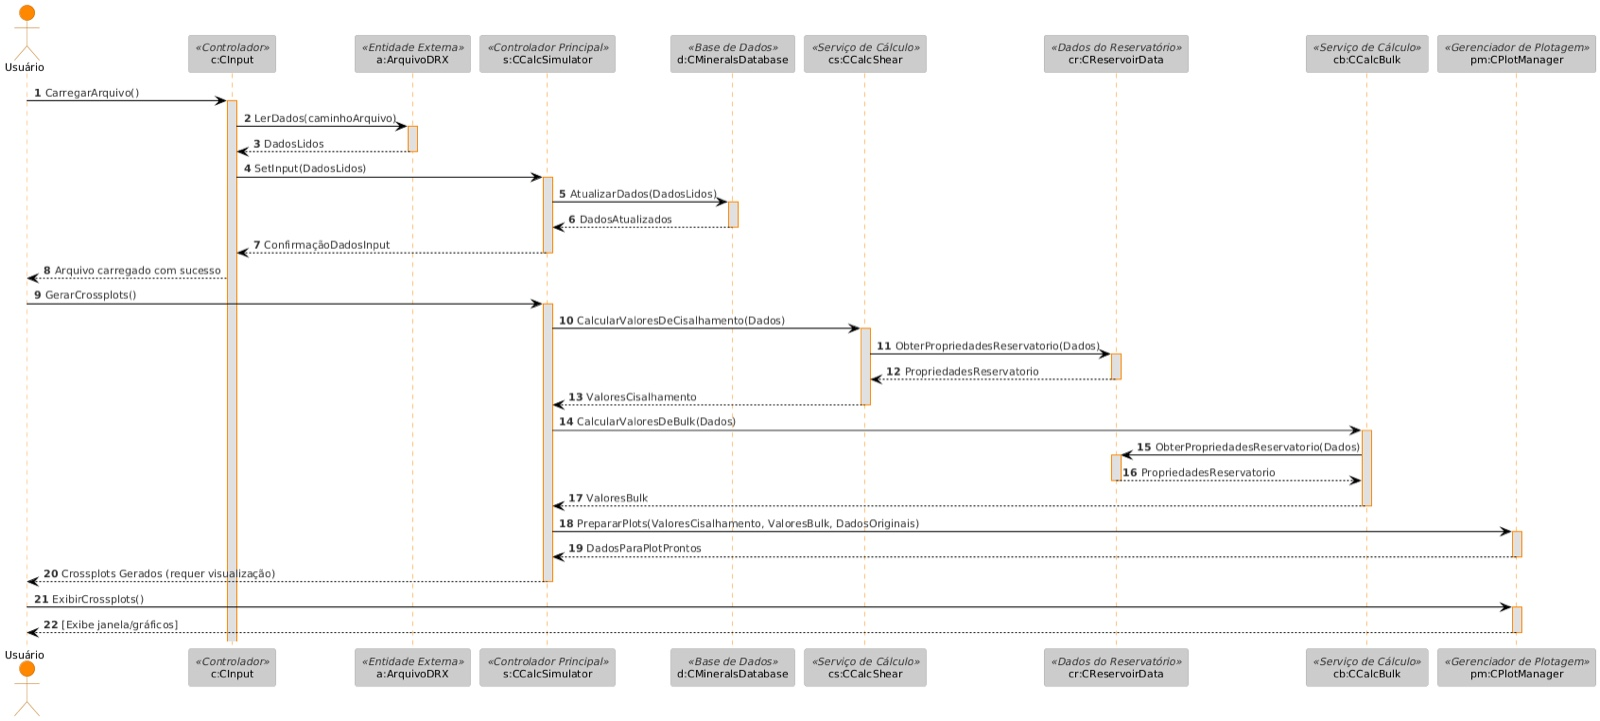
\includegraphics[width=1\textwidth]{imagens/SequenciaGeral.jpeg}
\par\end{centering}
\caption{Diagrama de seqüência geral\label{cap:Diagrama-de-sequencia}}
\end{figure}


\subsection{\textit{\emph{Diagrama de sequência específico\label{subsec: Diagrama de sequ=0000EAncia espec=0000EDfico}}}}

\begin{figure}[H]
\begin{centering}
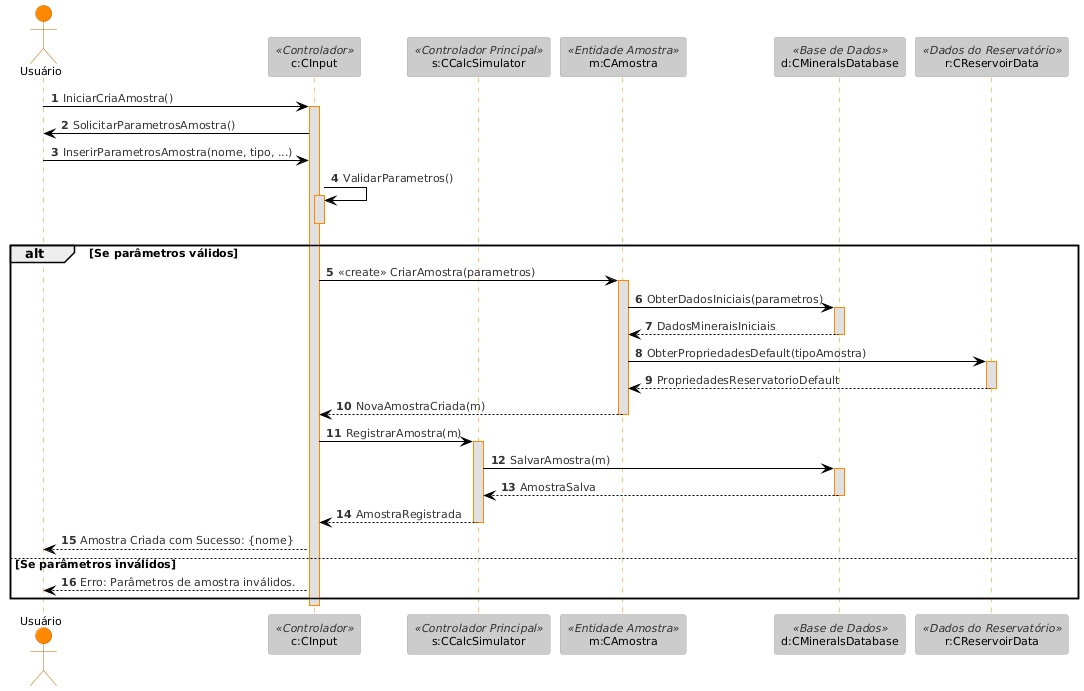
\includegraphics[width=1\textwidth]{imagens/SequenciaEspecifico.jpeg}
\par\end{centering}
\caption{Diagrama de seqüência específico\label{cap:Diagrama-de-sequencia-especifico}}
\end{figure}


\section{Diagrama de comunicação\index{comunicação} -- colaboração\index{colaboração}\label{subsec:Diagrama-de-Comunica=0000E7=0000E3o}\index{Diagrama de colaboração}\label{par:Diagrama-de-colabora=0000E7=0000E3o:} }

No diagrama de comunicação o foco é a interação e a troca de mensagens
e dados entre os objetos. 

Veja na Figura \ref{subsec:Diagrama-de-Comunica=0000E7=0000E3o} o
diagrama de comunicação mostrando a sequência de interação, onde a aplicação solicita leitura do arquivo da amostra para dar prosseguimento com o cálculo das propriedades, onde busca os dados do banco de dados. A aplicação armazena os dados e gera os resultados, e por fim solicita a geração dos gráficos de perfil.

\begin{figure}[H]
\begin{centering}
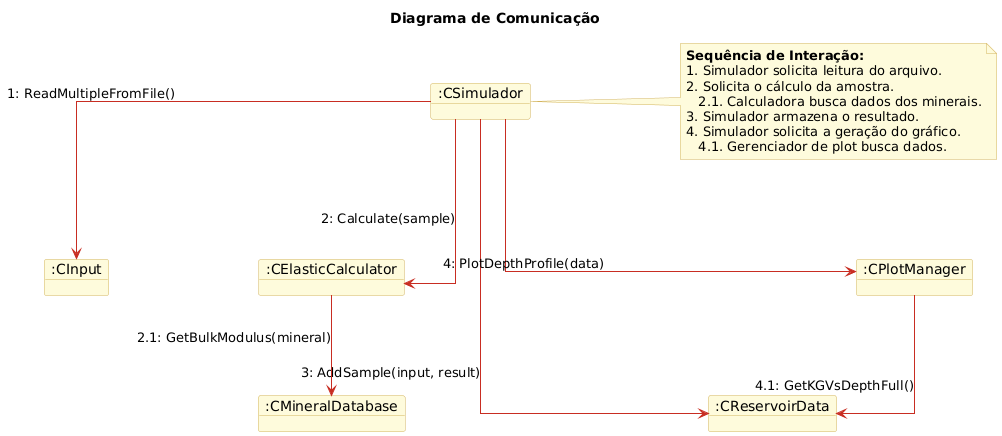
\includegraphics[width=1\textwidth]{imagens/Comunicacao.png}
\par\end{centering}
\caption{Diagrama de comunicação\label{cap:Diagrama-de-comunica=0000E7=0000E3o}}
\end{figure}


\section{Diagrama de estado\index{estado}\index{Diagrama de estado}\label{subsec:diagrama de estados}}


Veja na Figura \ref{cap:Diagrama-de-maquina-de-estado} o diagrama
de máquina de estado para o objeto CSimulador

\begin{figure}[H]
\begin{centering}
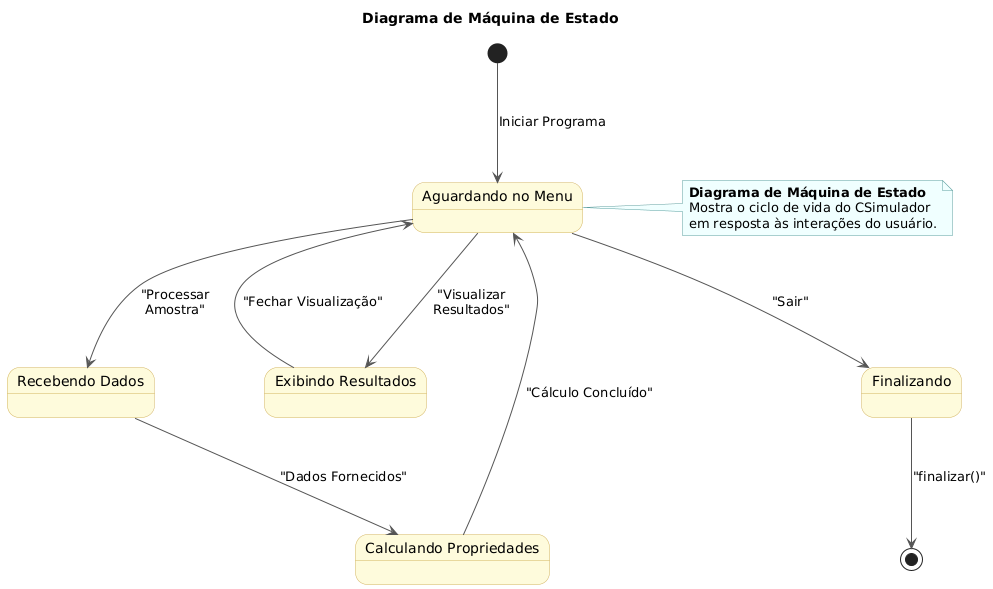
\includegraphics[width=1\textwidth]{imagens/MaquinaDeEstado.png}
\par\end{centering}
\caption{Diagrama de máquina de estado\label{cap:Diagrama-de-maquina-de-estado}}
\end{figure}


\section{Diagrama de atividades\label{sec: Diagrama de atividades}}

w

Veja na Figura \ref{cap:Diagrama-de-atividades} o diagrama de atividades. 

O processo se inicia no Nó Inicial, levando diretamente à primeira Atividade, que é "Apresentar Menu Principal". Neste ponto, uma decisão importante é oferecida ao usuário: se a opção for "Sair", o fluxo é desviado diretamente para a finalização do programa; caso contrário, ao escolher "Processar Amostra", o sistema avança para uma segunda decisão que define o método de entrada dos dados, seja através da atividade "Carregar de Arquivo" ou da criação manual. Uma vez que os dados da amostra são fornecidos por um desses caminhos, o fluxo converge e prossegue de forma sequencial para a fase de processamento, onde a atividade central de "Executar cálculos de propriedades poroelásticas" é realizada.

Com o término dos cálculos, indicado pelo estado "Resultados calculados e disponíveis", uma nova decisão permite ao usuário escolher entre "Gerar Gráficos" ou "Mostrar Relatórios" para a análise final. Concluída esta etapa, o diagrama chega ao seu ciclo de execução principal, onde a última decisão do fluxo pergunta se o usuário "Deseja realizar outra operação?". Uma resposta afirmativa reinicia todo o processo, retornando o controle ao menu principal para um novo ciclo de trabalho. Caso a resposta seja negativa, o fluxo segue para a atividade "Finalizar Software" e culmina no Nó Final, que representa o encerramento completo da aplicação.

\begin{figure}[H]
\begin{centering}
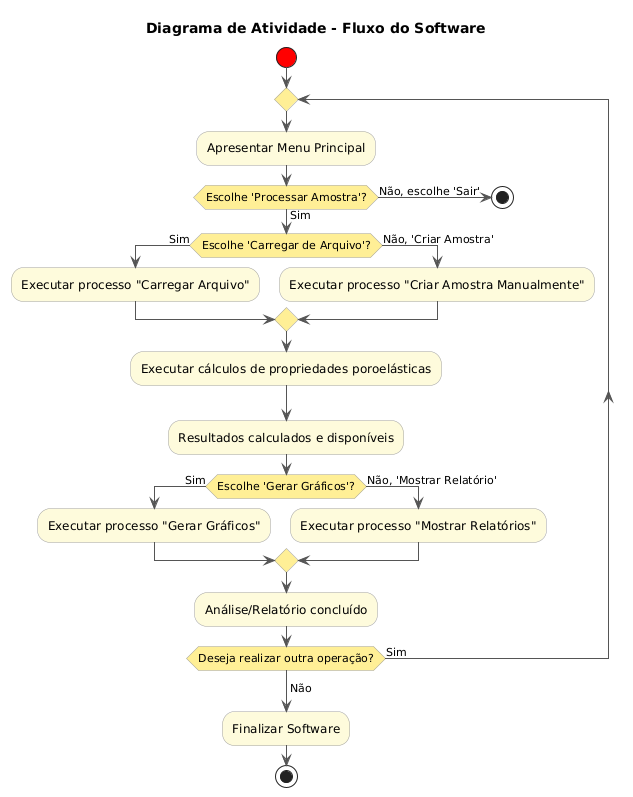
\includegraphics[width=1\textwidth]{imagens/Atividade-FluxoDoSoftware.png}
\par\end{centering}
\caption{Diagrama de atividades\label{cap:Diagrama-de-atividades}}
\end{figure}





\chapter{Projeto \label{chap:Projeto-do-Sistema}}

\lhead{\thechapter - Projeto} 

<<<<<<< HEAD
Neste capítulo do projeto de engenharia veremos questões associadas
ao projeto do sistema, incluindo protocolos, recursos, plataformas
suportadas, inplicações nos diagramas feitos anteriormente, diagramas
de componentes e implantação. Na segunda parte revisamos os diagramas
levando em conta as decisões do projeto do sistema.

\section{Projeto do Sistema\index{Projeto do sistema}\label{sec:Projeto-do-sistema}}

Depois da análise orientada a objeto desenvolve-se o projeto do sistema,
qual envolve etapas como a definição dos protocolos, da interface
API, o uso de recursos, a subdivisão do sistema em subsistemas, a
alocação dos subsistemas ao hardware e a seleção das estruturas de
controle, a seleção das plataformas do sistema, das bibliotecas externas,
dos padrões de projeto, além da tomada de decisões conceituais e políticas
que formam a infraestrutura do projeto.

Deve-se definir padrões de documentação, padrões para o nome das classes,
padrões de retorno e de parâmetros em métodos, características da
interface do usuário e características de desempenho. 

Segundo \cite{prog-UML-Rumbaugh,prog-UML-blaha}, o projeto do sistema
é a estratégia de alto nível para resolver o problema e elaborar uma
solução. Você deve se preocupar com itens como: 
=======
Neste cap�tulo do projeto de engenharia veremos quest�es associadas
ao projeto do sistema, incluindo protocolos, recursos, plataformas
suportadas, inplica��es nos diagramas feitos anteriormente, diagramas
de componentes e implanta��o. Na segunda parte revisamos os diagramas
levando em conta as decis�es do projeto do sistema.

\section{Projeto do Sistema\index{Projeto do sistema}\label{sec:Projeto-do-sistema}}

Depois da an�lise orientada a objeto desenvolve-se o projeto do sistema,
qual envolve etapas como a defini��o dos protocolos, da interface
API, o uso de recursos, a subdivis�o do sistema em subsistemas, a
aloca��o dos subsistemas ao hardware e a sele��o das estruturas de
controle, a sele��o das plataformas do sistema, das bibliotecas externas,
dos padr�es de projeto, al�m da tomada de decis�es conceituais e pol�ticas
que formam a infraestrutura do projeto.

Deve-se definir padr�es de documenta��o, padr�es para o nome das classes,
padr�es de retorno e de par�metros em m�todos, caracter�sticas da
interface do usu�rio e caracter�sticas de desempenho. 

Segundo \cite{prog-UML-Rumbaugh,prog-UML-blaha}, o projeto do sistema
� a estrat�gia de alto n�vel para resolver o problema e elaborar uma
solu��o. Voc� deve se preocupar com itens como: 
>>>>>>> 9cc8289ee257736c1a1b3309851f70a5b4b254e3
\begin{enumerate}
\item Protocolos\index{Protocolos}

\begin{itemize}
<<<<<<< HEAD
\item Definição dos protocolos de comunicação entre os diversos elementos
externos \\
(como dispositivos). Por exemplo: se o sistema envolve o uso dos nós
de um cluster, devem ser considerados aspectos como o protocolo de
comunicação entre os nós do cluster.
=======
\item Defini��o dos protocolos de comunica��o entre os diversos elementos
externos \\
(como dispositivos). Por exemplo: se o sistema envolve o uso dos n�s
de um cluster, devem ser considerados aspectos como o protocolo de
comunica��o entre os n�s do cluster.
>>>>>>> 9cc8289ee257736c1a1b3309851f70a5b4b254e3

\begin{itemize}
\item Neste projeto blablabla
\end{itemize}
<<<<<<< HEAD
\item Definição dos protocolos de comunicação entre os diversos elementos
=======
\item Defini��o dos protocolos de comunica��o entre os diversos elementos
>>>>>>> 9cc8289ee257736c1a1b3309851f70a5b4b254e3
internos \\
(como objetos). 

\begin{itemize}
\item Neste projeto blablabla
\end{itemize}
<<<<<<< HEAD
\item Definição da interface API de suas bibliotecas e sistemas.
=======
\item Defini��o da interface API de suas bibliotecas e sistemas.
>>>>>>> 9cc8289ee257736c1a1b3309851f70a5b4b254e3

\begin{itemize}
\item Neste projeto blablabla
\end{itemize}
<<<<<<< HEAD
\item Definição do formato dos arquivos gerados pelo software. Por exemplo:
=======
\item Defini��o do formato dos arquivos gerados pelo software. Por exemplo:
>>>>>>> 9cc8289ee257736c1a1b3309851f70a5b4b254e3
prefira formatos abertos, como arquivos txt e xml.

\begin{itemize}
\item Neste projeto blablabla
\end{itemize}
\end{itemize}
\item Recursos\index{Recursos}

\begin{itemize}
<<<<<<< HEAD
\item Identificação e alocação dos recursos globais, como os recursos do
sistema serão alocados, utilizados, compartilhados e liberados. Implicam
modificações no diagrama de componentes.
=======
\item Identifica��o e aloca��o dos recursos globais, como os recursos do
sistema ser�o alocados, utilizados, compartilhados e liberados. Implicam
modifica��es no diagrama de componentes.
>>>>>>> 9cc8289ee257736c1a1b3309851f70a5b4b254e3

\begin{itemize}
\item Neste projeto blablabla
\end{itemize}
<<<<<<< HEAD
\item Identificação da necessidade do uso de banco de dados. Implicam em
modificações nos diagramas de atividades e de componentes.
=======
\item Identifica��o da necessidade do uso de banco de dados. Implicam em
modifica��es nos diagramas de atividades e de componentes.
>>>>>>> 9cc8289ee257736c1a1b3309851f70a5b4b254e3

\begin{itemize}
\item Neste projeto blablabla
\end{itemize}
<<<<<<< HEAD
\item Identificação da necessidade de sistemas de armazenamento de massa.
=======
\item Identifica��o da necessidade de sistemas de armazenamento de massa.
>>>>>>> 9cc8289ee257736c1a1b3309851f70a5b4b254e3
Por exemplo: um \emph{storage} em um sistema de cluster ou sistemas
de backup.

\begin{itemize}
\item Neste projeto blablabla
\end{itemize}
\end{itemize}
\item Controle\index{Controle}

\begin{itemize}
<<<<<<< HEAD
\item Identificação e seleção da implementação de controle, seqüencial ou
concorrente, baseado em procedimentos ou eventos. Implicam modificações
no diagrama de execução. 
=======
\item Identifica��o e sele��o da implementa��o de controle, seq�encial ou
concorrente, baseado em procedimentos ou eventos. Implicam modifica��es
no diagrama de execu��o. 
>>>>>>> 9cc8289ee257736c1a1b3309851f70a5b4b254e3

\begin{itemize}
\item Neste projeto blablabla
\end{itemize}
<<<<<<< HEAD
\item Identificação das condições extremas e de prioridades.
=======
\item Identifica��o das condi��es extremas e de prioridades.
>>>>>>> 9cc8289ee257736c1a1b3309851f70a5b4b254e3

\begin{itemize}
\item Neste projeto blablabla
\end{itemize}
<<<<<<< HEAD
\item Identificação da necessidade de otimização. Por exemplo: prefira sistemas
com grande capacidade de memória; prefira vários hds pequenos a um
=======
\item Identifica��o da necessidade de otimiza��o. Por exemplo: prefira sistemas
com grande capacidade de mem�ria; prefira v�rios hds pequenos a um
>>>>>>> 9cc8289ee257736c1a1b3309851f70a5b4b254e3
grande.

\begin{itemize}
\item Neste projeto blablabla
\end{itemize}
<<<<<<< HEAD
\item Identificação e definição de \emph{loops} de controle e das escalas
=======
\item Identifica��o e defini��o de \emph{loops} de controle e das escalas
>>>>>>> 9cc8289ee257736c1a1b3309851f70a5b4b254e3
de tempo. 

\begin{itemize}
\item Neste projeto blablabla
\end{itemize}
<<<<<<< HEAD
\item Identificação de concorrências -- quais algoritmos podem ser implementados
=======
\item Identifica��o de concorr�ncias -- quais algoritmos podem ser implementados
>>>>>>> 9cc8289ee257736c1a1b3309851f70a5b4b254e3
usando processamento paralelo. 

\begin{itemize}
\item Neste projeto blablabla
\end{itemize}
\end{itemize}
\item Plataformas\index{Plataformas}

\begin{itemize}
<<<<<<< HEAD
\item Identificação das estruturas arquitetônicas comuns. 
=======
\item Identifica��o das estruturas arquitet�nicas comuns. 
>>>>>>> 9cc8289ee257736c1a1b3309851f70a5b4b254e3

\begin{itemize}
\item Neste projeto blablabla
\end{itemize}
<<<<<<< HEAD
\item Identificação de subsistemas relacionados à plataforma selecionada.
Podem implicar em modificações no diagrama de pacotes e no diagrama
=======
\item Identifica��o de subsistemas relacionados � plataforma selecionada.
Podem implicar em modifica��es no diagrama de pacotes e no diagrama
>>>>>>> 9cc8289ee257736c1a1b3309851f70a5b4b254e3
de componentes. 

\begin{itemize}
\item Neste projeto blablabla
\end{itemize}
<<<<<<< HEAD
\item Identificação e definição das plataformas a serem suportadas: hardware,
=======
\item Identifica��o e defini��o das plataformas a serem suportadas: hardware,
>>>>>>> 9cc8289ee257736c1a1b3309851f70a5b4b254e3
sistema operacional e linguagem de software.

\begin{itemize}
\item Neste projeto blablabla
\end{itemize}
<<<<<<< HEAD
\item Seleção das bibliotecas externas a serem utilizadas.
=======
\item Sele��o das bibliotecas externas a serem utilizadas.
>>>>>>> 9cc8289ee257736c1a1b3309851f70a5b4b254e3

\begin{itemize}
\item Neste projeto blablabla
\end{itemize}
<<<<<<< HEAD
\item Seleção da biblioteca utilizada para montar a interface gráfica do
=======
\item Sele��o da biblioteca utilizada para montar a interface gr�fica do
>>>>>>> 9cc8289ee257736c1a1b3309851f70a5b4b254e3
software -- GDI.

\begin{itemize}
\item Neste projeto blablabla
\end{itemize}
<<<<<<< HEAD
\item Seleção do ambiente de desenvolvimento para montar a interface de
=======
\item Sele��o do ambiente de desenvolvimento para montar a interface de
>>>>>>> 9cc8289ee257736c1a1b3309851f70a5b4b254e3
desenvolvimento -- IDE. 

\begin{itemize}
\item Neste projeto blablabla
\end{itemize}
\end{itemize}
<<<<<<< HEAD
\item Padrões de projeto

\begin{itemize}
\item Normalmente os padrões de projeto são identificados e passam a fazer
parte de uma biblioteca de padrões da empresa. Mas isto só ocorre
após a realização de diversos projetos.
=======
\item Padr�es de projeto

\begin{itemize}
\item Normalmente os padr�es de projeto s�o identificados e passam a fazer
parte de uma biblioteca de padr�es da empresa. Mas isto s� ocorre
ap�s a realiza��o de diversos projetos.
>>>>>>> 9cc8289ee257736c1a1b3309851f70a5b4b254e3

\begin{itemize}
\item Neste projeto blablabla
\end{itemize}
\end{itemize}
\end{enumerate}

\section{Projeto Orientado a Objeto -- POO\index{POO}\index{Projeto orientado a objeto}\label{sec:Projeto-orientado-a-objeto}}

<<<<<<< HEAD
O projeto orientado a objeto é a etapa posterior ao projeto do sistema.
Baseia-se na análise, mas considera as decisões do projeto do sistema.
Acrescenta a análise desenvolvida e as características da plataforma
escolhida (hardware, sistema operacional e linguagem de softwareção).
Passa pelo maior detalhamento do funcionamento do software, acrescentando
atributos e métodos que envolvem a solução de problemas específicos
não identificados durante a análise.

Envolve a otimização da estrutura de dados e dos algoritmos, a minimização
do tempo de execução, de memória e de custos. Existe um desvio de
ênfase para os conceitos da plataforma selecionada. 

Exemplo: na análise você define que existe um método para salvar um
arquivo em disco, define um atributo nomeDoArquivo, mas não se preocupa
com detalhes específicos da linguagem. Já no projeto, você inclui
as bibliotecas necessárias para acesso ao disco, cria um objeto específico
para acessar o disco, podendo, portanto, acrescentar novas classes
àquelas desenvolvidas na análise. 
=======
O projeto orientado a objeto � a etapa posterior ao projeto do sistema.
Baseia-se na an�lise, mas considera as decis�es do projeto do sistema.
Acrescenta a an�lise desenvolvida e as caracter�sticas da plataforma
escolhida (hardware, sistema operacional e linguagem de software��o).
Passa pelo maior detalhamento do funcionamento do software, acrescentando
atributos e m�todos que envolvem a solu��o de problemas espec�ficos
n�o identificados durante a an�lise.

Envolve a otimiza��o da estrutura de dados e dos algoritmos, a minimiza��o
do tempo de execu��o, de mem�ria e de custos. Existe um desvio de
�nfase para os conceitos da plataforma selecionada. 

Exemplo: na an�lise voc� define que existe um m�todo para salvar um
arquivo em disco, define um atributo nomeDoArquivo, mas n�o se preocupa
com detalhes espec�ficos da linguagem. J� no projeto, voc� inclui
as bibliotecas necess�rias para acesso ao disco, cria um objeto espec�fico
para acessar o disco, podendo, portanto, acrescentar novas classes
�quelas desenvolvidas na an�lise. 
>>>>>>> 9cc8289ee257736c1a1b3309851f70a5b4b254e3

\subsubsection{Efeitos do projeto no modelo\index{modelo} estrutural\label{subsec:Efeito-do-projeto-no-modelo-estrutural}}
\begin{itemize}
\item Adicionar nos diagramas de pacotes as bibliotecas e subsistemas selecionados
<<<<<<< HEAD
no projeto do sistema (exemplo: a biblioteca gráfica selecionada).
=======
no projeto do sistema (exemplo: a biblioteca gr�fica selecionada).
>>>>>>> 9cc8289ee257736c1a1b3309851f70a5b4b254e3

\begin{itemize}
\item Neste projeto blablabla
\end{itemize}
<<<<<<< HEAD
\item Novas classes e associações oriundas das bibliotecas selecionadas
=======
\item Novas classes e associa��es oriundas das bibliotecas selecionadas
>>>>>>> 9cc8289ee257736c1a1b3309851f70a5b4b254e3
e da linguagem escolhida devem ser acrescentadas ao modelo.

\begin{itemize}
\item Neste projeto blablabla
\end{itemize}
<<<<<<< HEAD
\item Estabelecer as dependências e restrições associadas à plataforma escolhida.
=======
\item Estabelecer as depend�ncias e restri��es associadas � plataforma escolhida.
>>>>>>> 9cc8289ee257736c1a1b3309851f70a5b4b254e3

\begin{itemize}
\item Neste projeto blablabla
\end{itemize}
\end{itemize}

<<<<<<< HEAD
\subsubsection{Efeitos do projeto no modelo\index{modelo} dinâmico\label{subsec:Efeito-do-projeto-no-modelo-dinamico}}
\begin{itemize}
\item Revisar os diagramas de seqüência e de comunicação considerando a
=======
\subsubsection{Efeitos do projeto no modelo\index{modelo} din�mico\label{subsec:Efeito-do-projeto-no-modelo-dinamico}}
\begin{itemize}
\item Revisar os diagramas de seq��ncia e de comunica��o considerando a
>>>>>>> 9cc8289ee257736c1a1b3309851f70a5b4b254e3
plataforma escolhida.

\begin{itemize}
\item Neste projeto blablabla
\end{itemize}
\item Verificar a necessidade de se revisar, ampliar e adicionar novos diagramas
<<<<<<< HEAD
de máquinas de estado e de atividades. 
=======
de m�quinas de estado e de atividades. 
>>>>>>> 9cc8289ee257736c1a1b3309851f70a5b4b254e3

\begin{itemize}
\item Neste projeto blablabla
\end{itemize}
\end{itemize}

\subsubsection{Efeitos do projeto nos atributos\index{atributos}\label{subsec:Efeito-do-projeto-nos-atributos}}
\begin{itemize}
\item Atributos novos podem ser adicionados a uma classe, como, por exemplo,
<<<<<<< HEAD
atributos específicos de uma determinada linguagem de softwareção
(acesso a disco, ponteiros, constantes e informações correlacionadas).
=======
atributos espec�ficos de uma determinada linguagem de software��o
(acesso a disco, ponteiros, constantes e informa��es correlacionadas).
>>>>>>> 9cc8289ee257736c1a1b3309851f70a5b4b254e3

\begin{itemize}
\item Neste projeto blablabla
\end{itemize}
\end{itemize}

<<<<<<< HEAD
\subsubsection{Efeitos do projeto nos métodos\index{métodos}\index{Efeitos do projeto nos métodos}}
\begin{itemize}
\item Em função da plataforma escolhida, verifique as possíveis alterações
nos métodos. O projeto do sistema costuma afetar os métodos de acesso
=======
\subsubsection{Efeitos do projeto nos m�todos\index{m�todos}\index{Efeitos do projeto nos m�todos}}
\begin{itemize}
\item Em fun��o da plataforma escolhida, verifique as poss�veis altera��es
nos m�todos. O projeto do sistema costuma afetar os m�todos de acesso
>>>>>>> 9cc8289ee257736c1a1b3309851f70a5b4b254e3
aos diversos dispositivos (exemplo: hd, rede).

\begin{itemize}
\item Neste projeto blablabla
\end{itemize}
<<<<<<< HEAD
\item De maneira geral os métodos devem ser divididos em dois tipos: i)
tomada de decisões, métodos políticos ou de controle; devem ser claros,
legíveis, flexíveis e usam polimorfismo. ii) realização de processamentos,
=======
\item De maneira geral os m�todos devem ser divididos em dois tipos: i)
tomada de decis�es, m�todos pol�ticos ou de controle; devem ser claros,
leg�veis, flex�veis e usam polimorfismo. ii) realiza��o de processamentos,
>>>>>>> 9cc8289ee257736c1a1b3309851f70a5b4b254e3
podem ser otimizados e em alguns casos o polimorfismo deve ser evitado.

\begin{itemize}
\item Neste projeto blablabla
\end{itemize}
<<<<<<< HEAD
\item Algoritmos complexos podem ser subdivididos. Verifique quais métodos
podem ser otimizados. Pense em utilizar algoritmos prontos como os
da STL (algoritmos genéricos).
=======
\item Algoritmos complexos podem ser subdivididos. Verifique quais m�todos
podem ser otimizados. Pense em utilizar algoritmos prontos como os
da STL (algoritmos gen�ricos).
>>>>>>> 9cc8289ee257736c1a1b3309851f70a5b4b254e3

\begin{itemize}
\item Neste projeto blablabla
\end{itemize}
<<<<<<< HEAD
\item Responda a pergunta: os métodos da classes estão dando resposta às
=======
\item Responda a pergunta: os m�todos da classes est�o dando resposta �s
>>>>>>> 9cc8289ee257736c1a1b3309851f70a5b4b254e3
responsabilidades da classe?

\begin{itemize}
\item Neste projeto blablabla
\end{itemize}
<<<<<<< HEAD
\item Revise os diagramas de classes, de seqüência e de máquina de estado.
=======
\item Revise os diagramas de classes, de seq��ncia e de m�quina de estado.
>>>>>>> 9cc8289ee257736c1a1b3309851f70a5b4b254e3

\begin{itemize}
\item Neste projeto blablabla
\end{itemize}
\end{itemize}

<<<<<<< HEAD
\subsubsection{Efeitos do projeto nas heranças\index{heranças}\index{Efeitos do projeto nas heranças}\index{Heranças}}
\begin{itemize}
\item Reorganização das classes e dos métodos (criar métodos genéricos com
parâmetros que nem sempre são necessários e englobam métodos existentes).
=======
\subsubsection{Efeitos do projeto nas heran�as\index{heran�as}\index{Efeitos do projeto nas heran�as}\index{Heran�as}}
\begin{itemize}
\item Reorganiza��o das classes e dos m�todos (criar m�todos gen�ricos com
par�metros que nem sempre s�o necess�rios e englobam m�todos existentes).
>>>>>>> 9cc8289ee257736c1a1b3309851f70a5b4b254e3

\begin{itemize}
\item Neste projeto blablabla
\end{itemize}
<<<<<<< HEAD
\item Abstração do comportamento comum (duas classes podem ter uma superclasse
=======
\item Abstra��o do comportamento comum (duas classes podem ter uma superclasse
>>>>>>> 9cc8289ee257736c1a1b3309851f70a5b4b254e3
em comum). 

\begin{itemize}
\item Neste projeto blablabla
\end{itemize}
<<<<<<< HEAD
\item Utilização de delegação para compartilhar a implementação (quando
você cria uma herança irreal para reaproveitar código). Usar com cuidado.
=======
\item Utiliza��o de delega��o para compartilhar a implementa��o (quando
voc� cria uma heran�a irreal para reaproveitar c�digo). Usar com cuidado.
>>>>>>> 9cc8289ee257736c1a1b3309851f70a5b4b254e3

\begin{itemize}
\item Neste projeto blablabla
\end{itemize}
<<<<<<< HEAD
\item Revise as heranças no diagrama de classes.
=======
\item Revise as heran�as no diagrama de classes.
>>>>>>> 9cc8289ee257736c1a1b3309851f70a5b4b254e3

\begin{itemize}
\item Neste projeto blablabla
\end{itemize}
\end{itemize}

<<<<<<< HEAD
\subsubsection{Efeitos do projeto nas associações\index{Efeitos do projeto nas associações}\index{Associações}}
\begin{itemize}
\item Deve-se definir na fase de projeto como as associações serão implementadas,
se obedecerão um determinado padrão ou não. 
=======
\subsubsection{Efeitos do projeto nas associa��es\index{Efeitos do projeto nas associa��es}\index{Associa��es}}
\begin{itemize}
\item Deve-se definir na fase de projeto como as associa��es ser�o implementadas,
se obedecer�o um determinado padr�o ou n�o. 
>>>>>>> 9cc8289ee257736c1a1b3309851f70a5b4b254e3

\begin{itemize}
\item Neste projeto blablabla
\end{itemize}
<<<<<<< HEAD
\item Se existe uma relação de \textquotedbl muitos\textquotedbl , pode-se
implementar a associação com a utilização de um dicionário, que é
um mapa das associações entre objetos. Assim, o objeto A acessa o
dicionário fornecendo uma chave (um nome para o objeto que deseja
acessar) e o dicionário retorna um valor (um ponteiro) para o objeto
=======
\item Se existe uma rela��o de \textquotedbl muitos\textquotedbl , pode-se
implementar a associa��o com a utiliza��o de um dicion�rio, que �
um mapa das associa��es entre objetos. Assim, o objeto A acessa o
dicion�rio fornecendo uma chave (um nome para o objeto que deseja
acessar) e o dicion�rio retorna um valor (um ponteiro) para o objeto
>>>>>>> 9cc8289ee257736c1a1b3309851f70a5b4b254e3
correto. 

\begin{itemize}
\item Neste projeto blablabla
\end{itemize}
<<<<<<< HEAD
\item Evite percorrer várias associações para acessar dados de classes distantes.
Pense em adicionar associações diretas.
=======
\item Evite percorrer v�rias associa��es para acessar dados de classes distantes.
Pense em adicionar associa��es diretas.
>>>>>>> 9cc8289ee257736c1a1b3309851f70a5b4b254e3

\begin{itemize}
\item Neste projeto blablabla
\end{itemize}
\end{itemize}

<<<<<<< HEAD
\subsubsection{Efeitos do projeto nas otimizações\index{otimizações}}
\begin{itemize}
\item Faça uma análise de aspectos relativos à otimização do sistema. Lembrando
que a otimização deve ser desenvolvida por analistas/desenvolvedores
=======
\subsubsection{Efeitos do projeto nas otimiza��es\index{otimiza��es}}
\begin{itemize}
\item Fa�a uma an�lise de aspectos relativos � otimiza��o do sistema. Lembrando
que a otimiza��o deve ser desenvolvida por analistas/desenvolvedores
>>>>>>> 9cc8289ee257736c1a1b3309851f70a5b4b254e3
experientes.

\begin{itemize}
\item Neste projeto blablabla
\end{itemize}
\item Identifique pontos a serem otimizados em que podem ser utilizados
processos concorrentes.

\begin{itemize}
\item Neste projeto blablabla
\end{itemize}
\item Pense em incluir bibliotecas otimizadas.
<<<<<<< HEAD
\item Se o acesso a determinados objetos (atributos/métodos) requer um caminho
longo (exemplo: A->B->C->D.atributo), pense em incluir associações
=======
\item Se o acesso a determinados objetos (atributos/m�todos) requer um caminho
longo (exemplo: A->B->C->D.atributo), pense em incluir associa��es
>>>>>>> 9cc8289ee257736c1a1b3309851f70a5b4b254e3
extras (exemplo: A-D.atributo).

\begin{itemize}
\item Neste projeto blablabla
\end{itemize}
<<<<<<< HEAD
\item Atributos auxiliares podem ser incluídos.
=======
\item Atributos auxiliares podem ser inclu�dos.
>>>>>>> 9cc8289ee257736c1a1b3309851f70a5b4b254e3

\begin{itemize}
\item Neste projeto blablabla
\end{itemize}
<<<<<<< HEAD
\item A ordem de execução pode ser alterada.
=======
\item A ordem de execu��o pode ser alterada.
>>>>>>> 9cc8289ee257736c1a1b3309851f70a5b4b254e3

\begin{itemize}
\item Neste projeto blablabla
\end{itemize}
<<<<<<< HEAD
\item Revise as associações nos diagramas de classes.
=======
\item Revise as associa��es nos diagramas de classes.
>>>>>>> 9cc8289ee257736c1a1b3309851f70a5b4b254e3

\begin{itemize}
\item Neste projeto blablabla
\end{itemize}
\end{itemize}
<<<<<<< HEAD
Depois de revisados os diagramas da análise você pode montar dois
diagramas relacionados à infraestrutura do sistema. As dependências
dos arquivos e bibliotecas podem ser descritos pelo diagrama de componentes,
e as relações e dependências entre o sistema e o hardware podem ser
ilustradas com o diagrama de implantação.
=======
Depois de revisados os diagramas da an�lise voc� pode montar dois
diagramas relacionados � infraestrutura do sistema. As depend�ncias
dos arquivos e bibliotecas podem ser descritos pelo diagrama de componentes,
e as rela��es e depend�ncias entre o sistema e o hardware podem ser
ilustradas com o diagrama de implanta��o.
>>>>>>> 9cc8289ee257736c1a1b3309851f70a5b4b254e3

\section{Diagrama de Componentes\index{Diagrama de componentes}\label{sec:Diagrama-de-componentes}}

O diagrama de componentes mostra a forma como os componentes do software
<<<<<<< HEAD
se relacionam, suas dependências. Inclui itens como: componentes,
subsistemas, executáveis, nós, associações, dependências, generalizações,
restrições e notas. Exemplos de componentes são bibliotecas estáticas,
bibliotecas dinâmicas, dlls, componentes Java, executáveis, arquivos
de disco, código-fonte. 

Veja na Figura \ref{cap:Diagrama-de-componentes} um exemplo de diagrama
de componentes. Observe que este inclui muitas dependências, ilustrando
as relações entre os arquivos. Por exemplo: o subsistema biblioteca
inclui os arquivos das classes A e B, e a geração dos objetos A.obj
e B.obj depende dos arquivos A.h, A.cpp, B.h e B.cpp. A geração da
biblioteca depende dos arquivos A.obj e B.obj. O subsistema biblioteca
Qt, um subsistema exerno, inclui os arquivos de código da biblioteca
Qt e a biblioteca em si. O subsistema banco de dados representa o
banco de dados utilizado pelo sistema e tem uma interface de acesso
que é utilizada pelo software para acesso aos dados armazenados no
banco de dados. O software executável a ser gerado depende da biblioteca
gerada, dos arquivos da biblioteca Qt, do módulo de arquivos MinhaJanela
e do banco de dados.

Algumas observações úteis para o diagrama de componentes:
\begin{itemize}
\item De posse do diagrama de componentes, temos a lista de todos os arquivos
necessários para compilar e rodar o software.
\item Observe que um assunto/pacote pode se transformar em uma biblioteca
e será incluído no diagrama de componentes.
\item A ligação entre componentes pode incluir um estereótipo indicando
=======
se relacionam, suas depend�ncias. Inclui itens como: componentes,
subsistemas, execut�veis, n�s, associa��es, depend�ncias, generaliza��es,
restri��es e notas. Exemplos de componentes s�o bibliotecas est�ticas,
bibliotecas din�micas, dlls, componentes Java, execut�veis, arquivos
de disco, c�digo-fonte. 

Veja na Figura \ref{cap:Diagrama-de-componentes} um exemplo de diagrama
de componentes. Observe que este inclui muitas depend�ncias, ilustrando
as rela��es entre os arquivos. Por exemplo: o subsistema biblioteca
inclui os arquivos das classes A e B, e a gera��o dos objetos A.obj
e B.obj depende dos arquivos A.h, A.cpp, B.h e B.cpp. A gera��o da
biblioteca depende dos arquivos A.obj e B.obj. O subsistema biblioteca
Qt, um subsistema exerno, inclui os arquivos de c�digo da biblioteca
Qt e a biblioteca em si. O subsistema banco de dados representa o
banco de dados utilizado pelo sistema e tem uma interface de acesso
que � utilizada pelo software para acesso aos dados armazenados no
banco de dados. O software execut�vel a ser gerado depende da biblioteca
gerada, dos arquivos da biblioteca Qt, do m�dulo de arquivos MinhaJanela
e do banco de dados.

Algumas observa��es �teis para o diagrama de componentes:
\begin{itemize}
\item De posse do diagrama de componentes, temos a lista de todos os arquivos
necess�rios para compilar e rodar o software.
\item Observe que um assunto/pacote pode se transformar em uma biblioteca
e ser� inclu�do no diagrama de componentes.
\item A liga��o entre componentes pode incluir um estere�tipo indicando
>>>>>>> 9cc8289ee257736c1a1b3309851f70a5b4b254e3
o tipo de relacionamento ou algum protocolo utilizado.
\end{itemize}
Neste projeto blablabla

\begin{figure}[H]
\begin{centering}

\includegraphics[width=1\textwidth]{imagens/DiagramaDeComponentes-Assuntos-Pacotes}
\par\end{centering}
\caption{Diagrama de componentes\label{cap:Diagrama-de-componentes}}
\end{figure}


<<<<<<< HEAD
\section{Diagrama de Implantação\index{Diagrama de implantação}\index{Diagrama de execução}\label{sec:Diagrama-de-execu=0000E7=0000E3o}}

O diagrama de implantação é um diagrama de alto nível que inclui relações
entre o sistema e o hardware e que se preocupa com os aspectos da
arquitetura computacional escolhida. Seu enfoque é o hardware, a configuração
dos nós em tempo de execução. 

O diagrama de implantação deve incluir os elementos necessários para
que o sistema seja colocado em funcionamento: computador, periféricos,
processadores, dispositivos, nós, relacionamentos de dependência,
associação, componentes, subsistemas, restrições e notas.

Veja na Figura \ref{cap:Diagrama-de-implanta=0000E7=0000E3o.} um
exemplo de diagrama de implantação de um cluster. Observe a presença
de um servidor conectado a um switch. Os nós do cluster (ou clientes)
também estão conectados ao switch. Os resultados das simulações são
armazenados em um servidor de arquivos (\emph{storage}).

Pode-se utilizar uma anotação de localização para identificar onde
determinado componente está residente, por exemplo \{localização:
=======
\section{Diagrama de Implanta��o\index{Diagrama de implanta��o}\index{Diagrama de execu��o}\label{sec:Diagrama-de-execu=0000E7=0000E3o}}

O diagrama de implanta��o � um diagrama de alto n�vel que inclui rela��es
entre o sistema e o hardware e que se preocupa com os aspectos da
arquitetura computacional escolhida. Seu enfoque � o hardware, a configura��o
dos n�s em tempo de execu��o. 

O diagrama de implanta��o deve incluir os elementos necess�rios para
que o sistema seja colocado em funcionamento: computador, perif�ricos,
processadores, dispositivos, n�s, relacionamentos de depend�ncia,
associa��o, componentes, subsistemas, restri��es e notas.

Veja na Figura \ref{cap:Diagrama-de-implanta=0000E7=0000E3o.} um
exemplo de diagrama de implanta��o de um cluster. Observe a presen�a
de um servidor conectado a um switch. Os n�s do cluster (ou clientes)
tamb�m est�o conectados ao switch. Os resultados das simula��es s�o
armazenados em um servidor de arquivos (\emph{storage}).

Pode-se utilizar uma anota��o de localiza��o para identificar onde
determinado componente est� residente, por exemplo \{localiza��o:
>>>>>>> 9cc8289ee257736c1a1b3309851f70a5b4b254e3
sala 3\}.

\begin{figure}[H]
\begin{centering}
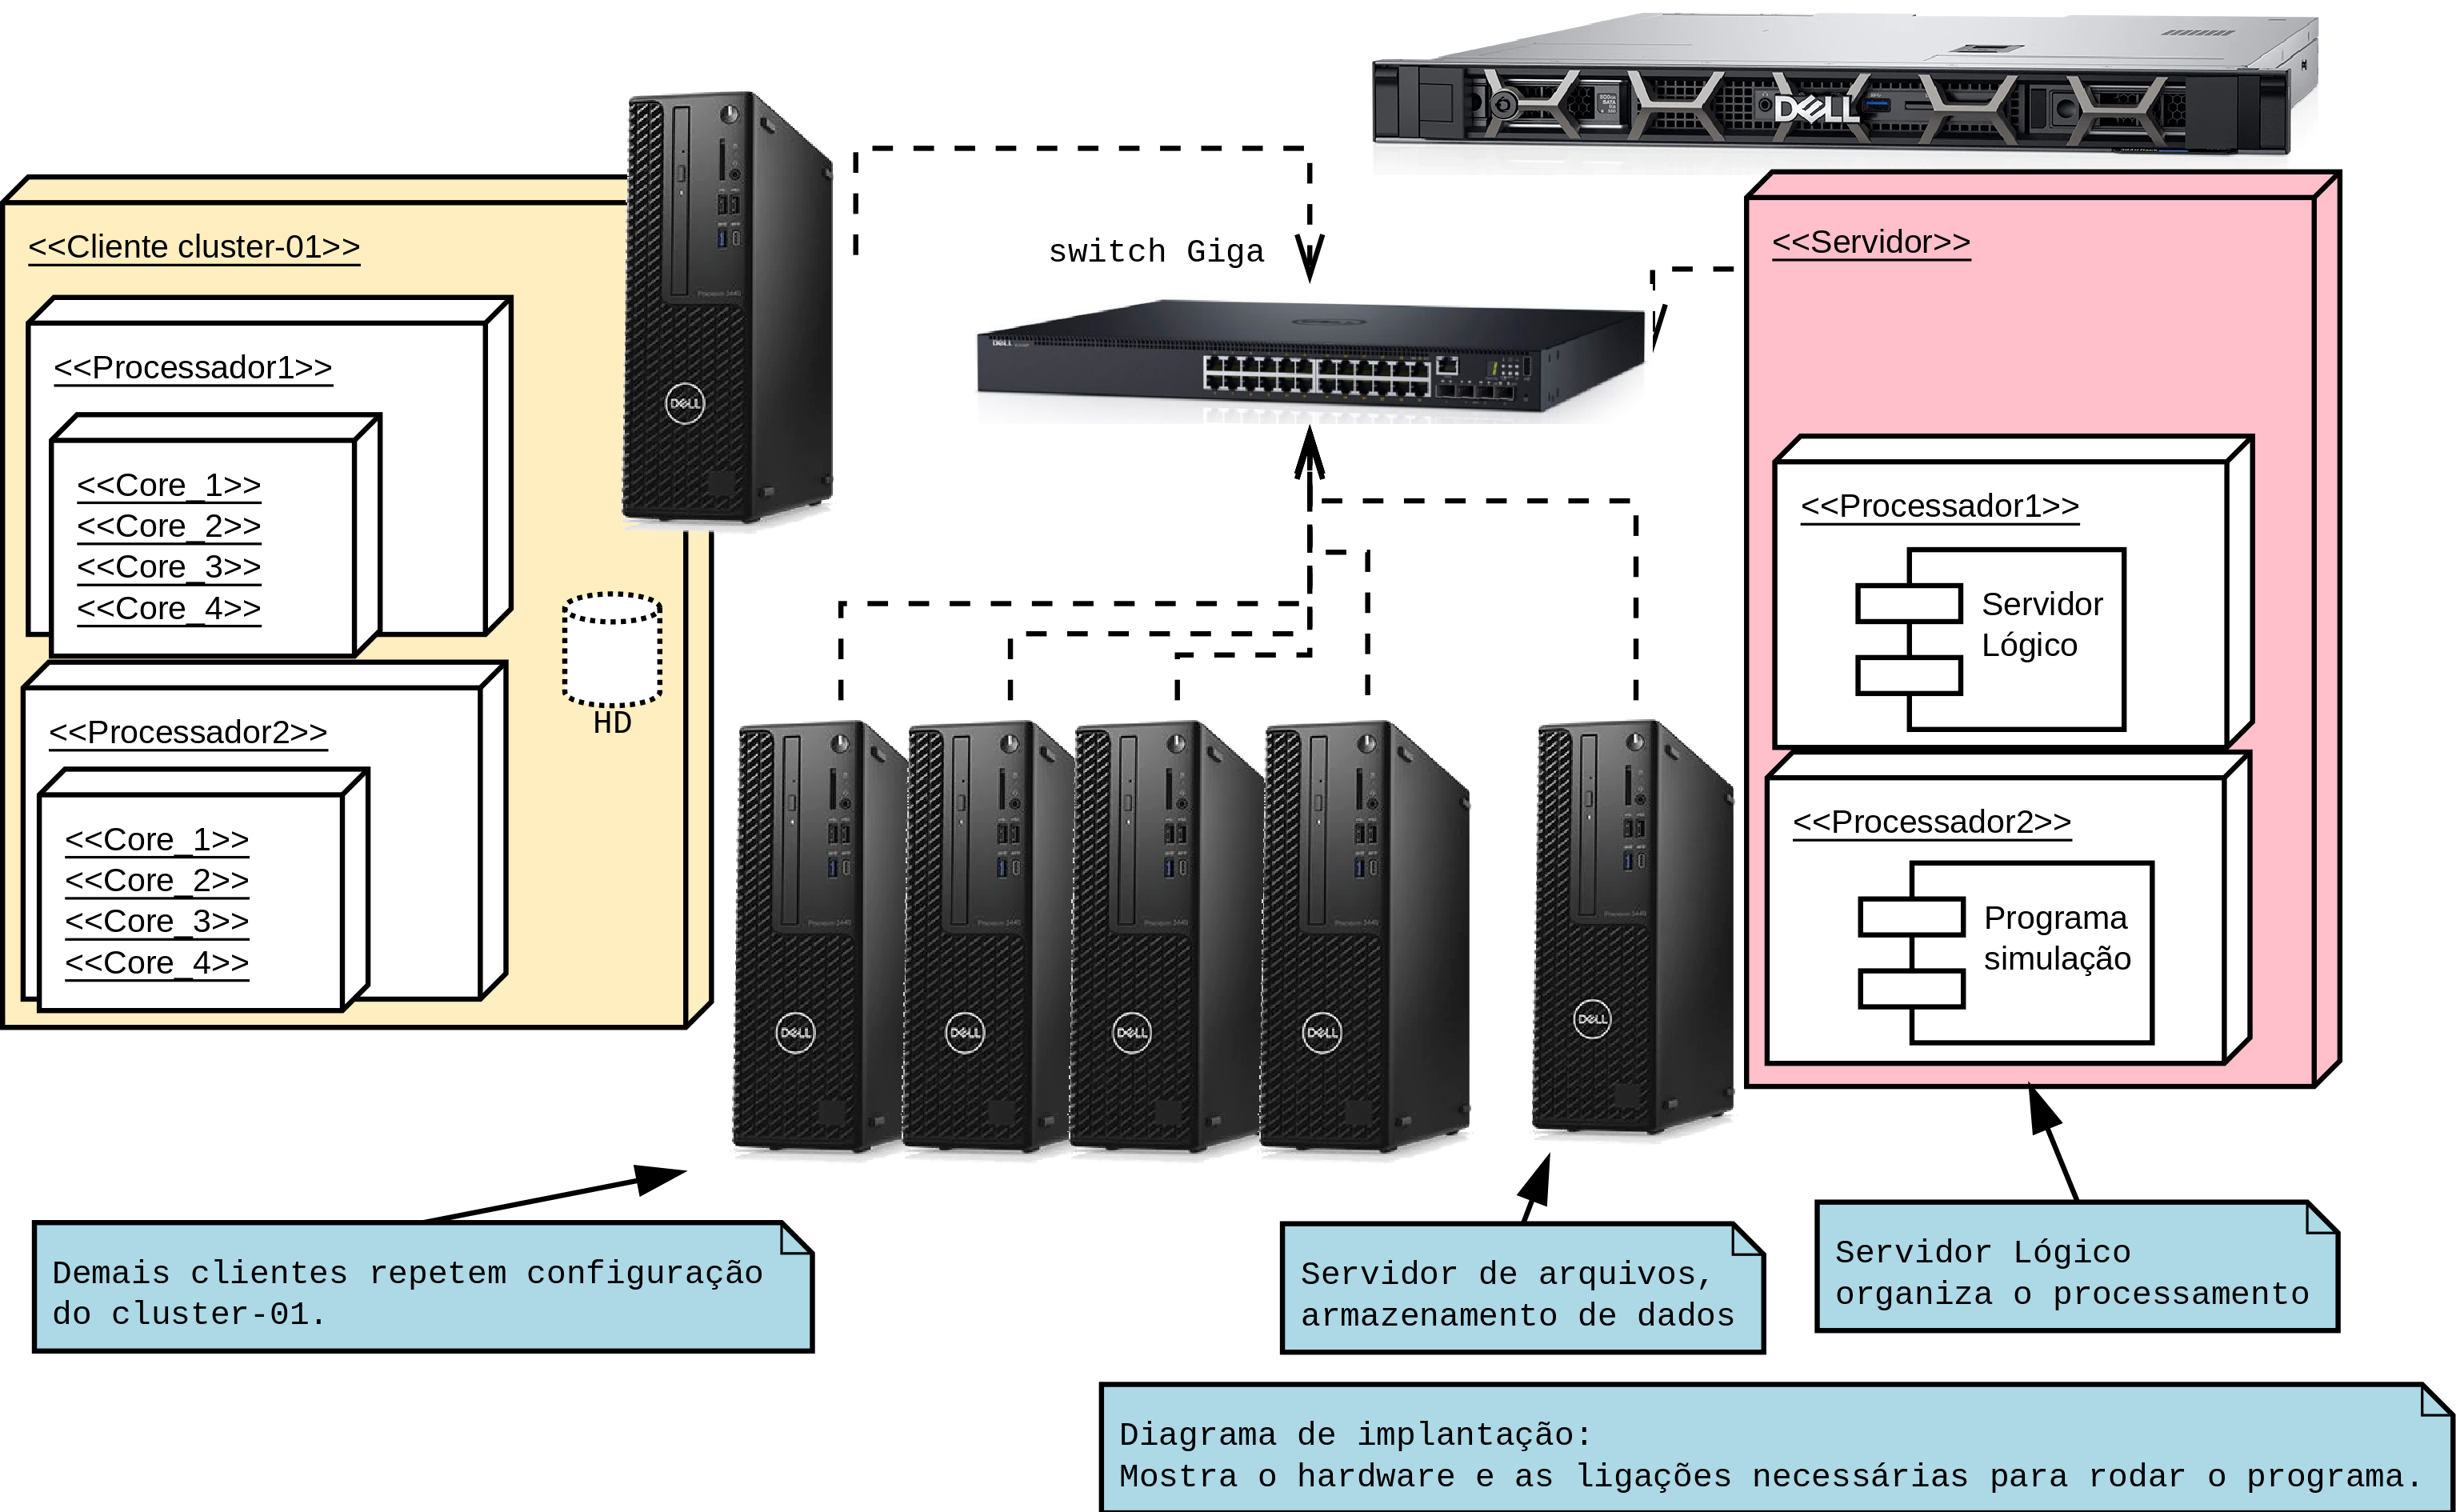
\includegraphics[width=1\textwidth]{imagens/DiagramaDeExecucao}
\par\end{centering}
<<<<<<< HEAD
\caption{Diagrama de implantação\label{cap:Diagrama-de-implanta=0000E7=0000E3o.}}
=======
\caption{Diagrama de implanta��o\label{cap:Diagrama-de-implanta=0000E7=0000E3o.}}
>>>>>>> 9cc8289ee257736c1a1b3309851f70a5b4b254e3
\end{figure}

\begin{description}
\item [{Nota:}] ~\\
<<<<<<< HEAD
Não perca de vista a visão do todo; do projeto de engenharia como
um todo. Cada capítulo, cada seção, cada parágrafo deve se encaixar.
Este é um diferencial fundamental do engenheiro em relação ao técnico,
=======
N�o perca de vista a vis�o do todo; do projeto de engenharia como
um todo. Cada cap�tulo, cada se��o, cada par�grafo deve se encaixar.
Este � um diferencial fundamental do engenheiro em rela��o ao t�cnico,
>>>>>>> 9cc8289ee257736c1a1b3309851f70a5b4b254e3
a capacidade de desenvolver projetos, de ver o todo e suas diferentes
partes, de modelar processos/sistemas/produtos de engenharia.
\end{description}




<<<<<<< HEAD
\chapter{Lista das Características/\emph{Features}\label{chap:Lista-das-Caracter=0000EDsticas}}

Neste capítulo lista-se as características do sistema a ser desenvolvido
(seção \ref{sec:Lista-de-caracter=0000EDsticas}). 

\section{Lista de características <\textcompwordmark <features>\textcompwordmark >\label{sec:Lista-de-caracter=0000EDsticas}}

No final do ciclo de concepção e análise chegamos a uma lista de características
<\textcompwordmark <\emph{features}>\textcompwordmark > que teremos
de implementar.

Após a análises desenvolvidas e considerando o requisito de que este
material deve ter um formato didático, chegamos a seguinte lista:
\begin{itemize}
\item v0.1
\begin{itemize}
\item Ex: O sistema deve plotar gráficos de pressão x temperatura
=======
\chapter{Lista das Caracter�sticas/\emph{Features}\label{chap:Lista-das-Caracter=0000EDsticas}}

Neste cap�tulo lista-se as caracter�sticas do sistema a ser desenvolvido
(se��o \ref{sec:Lista-de-caracter=0000EDsticas}). 

\section{Lista de caracter�sticas <\textcompwordmark <features>\textcompwordmark >\label{sec:Lista-de-caracter=0000EDsticas}}

No final do ciclo de concep��o e an�lise chegamos a uma lista de caracter�sticas
<\textcompwordmark <\emph{features}>\textcompwordmark > que teremos
de implementar.

Ap�s a an�lises desenvolvidas e considerando o requisito de que este
material deve ter um formato did�tico, chegamos a seguinte lista:
\begin{itemize}
\item v0.1
\begin{itemize}
\item Ex: O sistema deve plotar gr�ficos de press�o x temperatura
>>>>>>> 9cc8289ee257736c1a1b3309851f70a5b4b254e3
\item Ex: O sistema deve permitir abrir arquivos num formato especificado.
\item Ex: nome de classe a ser implementada e testada
\end{itemize}
\item v0.3
\begin{itemize}
\item Lista de classes a serem implementadas
\item Testes
\end{itemize}
\item v0.7
\begin{itemize}
\item Lista de classes a serem implementadas
\item Testes
\end{itemize}
\end{itemize}



<<<<<<< HEAD
\noindent\lhead{Referências} \chead{} \rhead{}\bibliographystyle{apalike}
=======
\noindent\lhead{Refer�ncias} \chead{} \rhead{}\bibliographystyle{apalike}
>>>>>>> 9cc8289ee257736c1a1b3309851f70a5b4b254e3
\bibliography{bibliografia}

\appendix

\chapter{Modelagem Matemática e Algoritmos de Cálculo}
\lhead{Apêndice \thechapter: Modelagem Matemática e Algoritmos}\rhead{\thepage}

Descreve-se neste apêndice o detalhamento dos modelos matemáticos utilizados para a estimativa das propriedades elásticas efetivas do compósito rochoso, bem como o algoritmo central que implementa estes cálculos no sistema desenvolvido. Este material, embora fundamental para a reprodutibilidade e compreensão profunda dos resultados, é apresentado aqui por seu elevado nível de detalhe técnico.

\section{Modelos de Média Poroelástica}

Para estimar as propriedades elásticas de uma rocha (um material compósito), a partir das propriedades de seus minerais constituintes, foram empregados os modelos de média de Voigt, Reuss e Hill. Estes modelos fornecem, respectivamente, os limites superior e inferior, e uma média empírica para os módulos elásticos efetivos.

Dada uma rocha composta por $N$ minerais, onde cada mineral $i$ possui uma fração volumétrica $f_i$, um módulo de compressibilidade $K_i$ e um módulo de cisalhamento $G_i$, os módulos efetivos do compósito ($K_{eff}$, $G_{eff}$) são calculados da seguinte forma:

\paragraph{Média de Voigt (Limite Superior)}
Este modelo assume que todos os constituintes sofrem a mesma deformação.
\begin{equation}
    K_{Voigt} = \sum_{i=1}^{N} f_i K_i
\end{equation}
\begin{equation}
    G_{Voigt} = \sum_{i=1}^{N} f_i G_i
\end{equation}

\paragraph{Média de Reuss (Limite Inferior)}
Este modelo assume que todos os constituintes estão sujeitos à mesma tensão.
\begin{equation}
    K_{Reuss} = \left( \sum_{i=1}^{N} \frac{f_i}{K_i} \right)^{-1}
\end{equation}
\begin{equation}
    G_{Reuss} = \left( \sum_{i=1}^{N} \frac{f_i}{G_i} \right)^{-1}
\end{equation}

\paragraph{Média de Voigt-Reuss-Hill}
Considerada uma aproximação empírica mais realista, é a média aritmética simples dos limites de Voigt e Reuss.
\begin{equation}
    K_{Hill} = \frac{K_{Voigt} + K_{Reuss}}{2}
\end{equation}
\begin{equation}
    G_{Hill} = \frac{G_{Voigt} + G_{Reuss}}{2}
\end{equation}

\section{Algoritmo de Cálculo dos Módulos Elásticos}

O núcleo de processamento do sistema, encapsulado na classe \texttt{CElasticCalculator}, segue um algoritmo bem definido para determinar as propriedades de uma amostra. O processo pode ser descrito em alto nível pelo seguinte pseudocódigo:

\begin{verbatim}
FUNÇÃO Calculate(amostra):
    // 1. Calcula os módulos de compressibilidade (K)
    k_voigt = m_bulkCalc.CalculateVoigt(amostra)
    k_reuss = m_bulkCalc.CalculateReuss(amostra)
    k_hill = (k_voigt + k_reuss) / 2.0
    
    // 2. Calcula os módulos de cisalhamento (G)
    g_voigt = m_shearCalc.CalculateVoigt(amostra)
    g_reuss = m_shearCalc.CalculateReuss(amostra)
    g_hill = (g_voigt + g_reuss) / 2.0
    
    // 3. Agrega e retorna os resultados
    RETORNE um objeto Result contendo:
        k_voigt, k_reuss, k_hill,
        g_voigt, g_reuss, g_hill
FIM FUNÇÃO
\end{verbatim}
Este algoritmo demonstra a delegação de responsabilidades no sistema: a classe \texttt{CElasticCalculator} orquestra o cálculo, enquanto as classes \texttt{CBulkCalculator} e \texttt{CShearCalculator} realizam os cálculos específicos para cada módulo, acessando a base de dados de minerais conforme a necessidade.



\chapter{Código-Fonte Selecionado}
\lhead{Apêndice \thechapter: Código-Fonte Selecionado}\rhead{\thepage}

Este apêndice apresenta o código-fonte das interfaces (arquivos de cabeçalho \texttt{.h}) das principais classes desenvolvidas no projeto. A escolha por apresentar as interfaces visa a oferecer uma visão clara e concisa da arquitetura orientada a objeto, das responsabilidades de cada classe e de suas inter-relações, sem o detalhamento excessivo dos arquivos de implementação.

\section{Classe CSimulador}
Responsável pela orquestração geral do sistema, gerenciando o fluxo de execução e a interação entre os componentes.
\begin{verbatim}
#ifndef CPECAPPLICATION_H
#define CPECAPPLICATION_H

#include "CInput.h"
#include "CElasticCalculator.h"
#include "CMineralDatabase.h"
#include "CReservoirData.h"
#include "CPlotManager.h"

class CSimulador {
public:
    CSimulador();
    void Run();

private:
    CInput m_inputManager;
    CMineralDatabase m_database;
    CElasticCalculator m_calculator;
    CReservoirData m_reservoirData;
    CPlotManager m_plotManager;
    bool m_running;

    void Menu();
    void Initialize();
    void Finalize();
};

#endif
\end{verbatim}

\section{Classe CElasticCalculator}
Encapsula a lógica de cálculo dos módulos elásticos, utilizando composição para delegar os cálculos específicos.
\begin{verbatim}
#ifndef CELASTICCALCULATOR_H
#define CELASTICCALCULATOR_H

#include "CMineralDatabase.h"
#include "CAmostra.h"
#include "CBulkCalculator.h"
#include "CShearCalculator.h"

class CElasticCalculator {
public:
    struct Result {
        float bulkVoigt, bulkReuss, bulkHill;
        float shearVoigt, shearReuss, shearHill;
    };

    explicit CElasticCalculator(const CMineralDatabase& db);
    Result Calculate(const CAmostra& amostra) const;

private:
    CBulkCalculator m_bulkCalc;
    CShearCalculator m_shearCalc;
};

#endif // CELASTICCALCULATOR_H
\end{verbatim}

\section{Classe CAmostra}
Representa a entidade de dados de uma amostra de rocha, encapsulando todas as suas propriedades.
\begin{verbatim}
#ifndef CAMOSTRA_H
#define CAMOSTRA_H

#include <string>
#include <map>

class CAmostra {
public:
    CAmostra();
    CAmostra(const std::string& reservatorio, const std::string& nome,
             float profundidade, float porosidade,
             const std::map<std::string, float>& minerais);

    const std::string& NomeReservatorio() const;
    const std::string& NomeAmostra() const;
    float Profundidade() const;
    float Porosidade() const;
    const std::map<std::string, float>& Minerais() const;

private:
    std::string m_reservatorio;
    std::string m_nome;
    float m_profundidade;
    float m_porosidade;
    std::map<std::string, float> m_minerais;
};

#endif
\end{verbatim}

\printindex
\end{document}
